\section{Adaptive dynamics: Can actions of accreted globular clusters constrain the gravitational potential?}
\subsection{Integrals of motion}

\subsubsection{Energy and angular momentum}
\subsubsection{Actions}
\begin{itemize}
    \item General action introduction (heuristic / properly)
    \item explain Staeckel fudge
    \item mention galpy
    
\end{itemize}
\subsection{Merger tree}
figure: Merger tree of Auriga 24. 
\subsection{Globular cluster sample selection}
Due to the resolution of the simulation, $\rm{M} = 5 \cdot 10 ^ 4\ M_{\odot}$, we set one stellar particle as one \ac{GC}. We find the three biggest \ac{DG} merger events in the merger tree. All stellar particles which were accreted by the main halo are followed through the evolution and kept as accreted \acp{GC} as long as they do not cross the disk in a sense that they either are directly in the disk - defined per snapshot as within the radius $\rm{R}_d \<= 0.1 \ R_{200}$ and the height $\rm{z}_d = 0.03\ R_d$ to match the \ac{MW} disk's height in the $z = 0$ snapshot - or changed signs between successive snapshots while being inside the disk radius since we assume that in these cases the \ac{GC} would be disrupted. 


\begin{table}[htbp]
    \centering
    \begin{tabular}{c|c|c|c|c}
         \makecell{name}& \makecell{Merger time}& \makecell{mass of \ac{DG}\\ at merger} & \makecell{num of \\accreted particles} & \makecell{mass of \\accreted particles}\\
         \hline
         prog2& & &&\\
         prog3& & &&\\
         prog4& & &&
    \end{tabular}
    \caption{Progenitor parameters}
    \label{tab:prog_overview}
\end{table}


\begin{figure}[htbp]
    \centering
    \begin{subfigure}[c]{0.45\textwidth}
    \centering
    	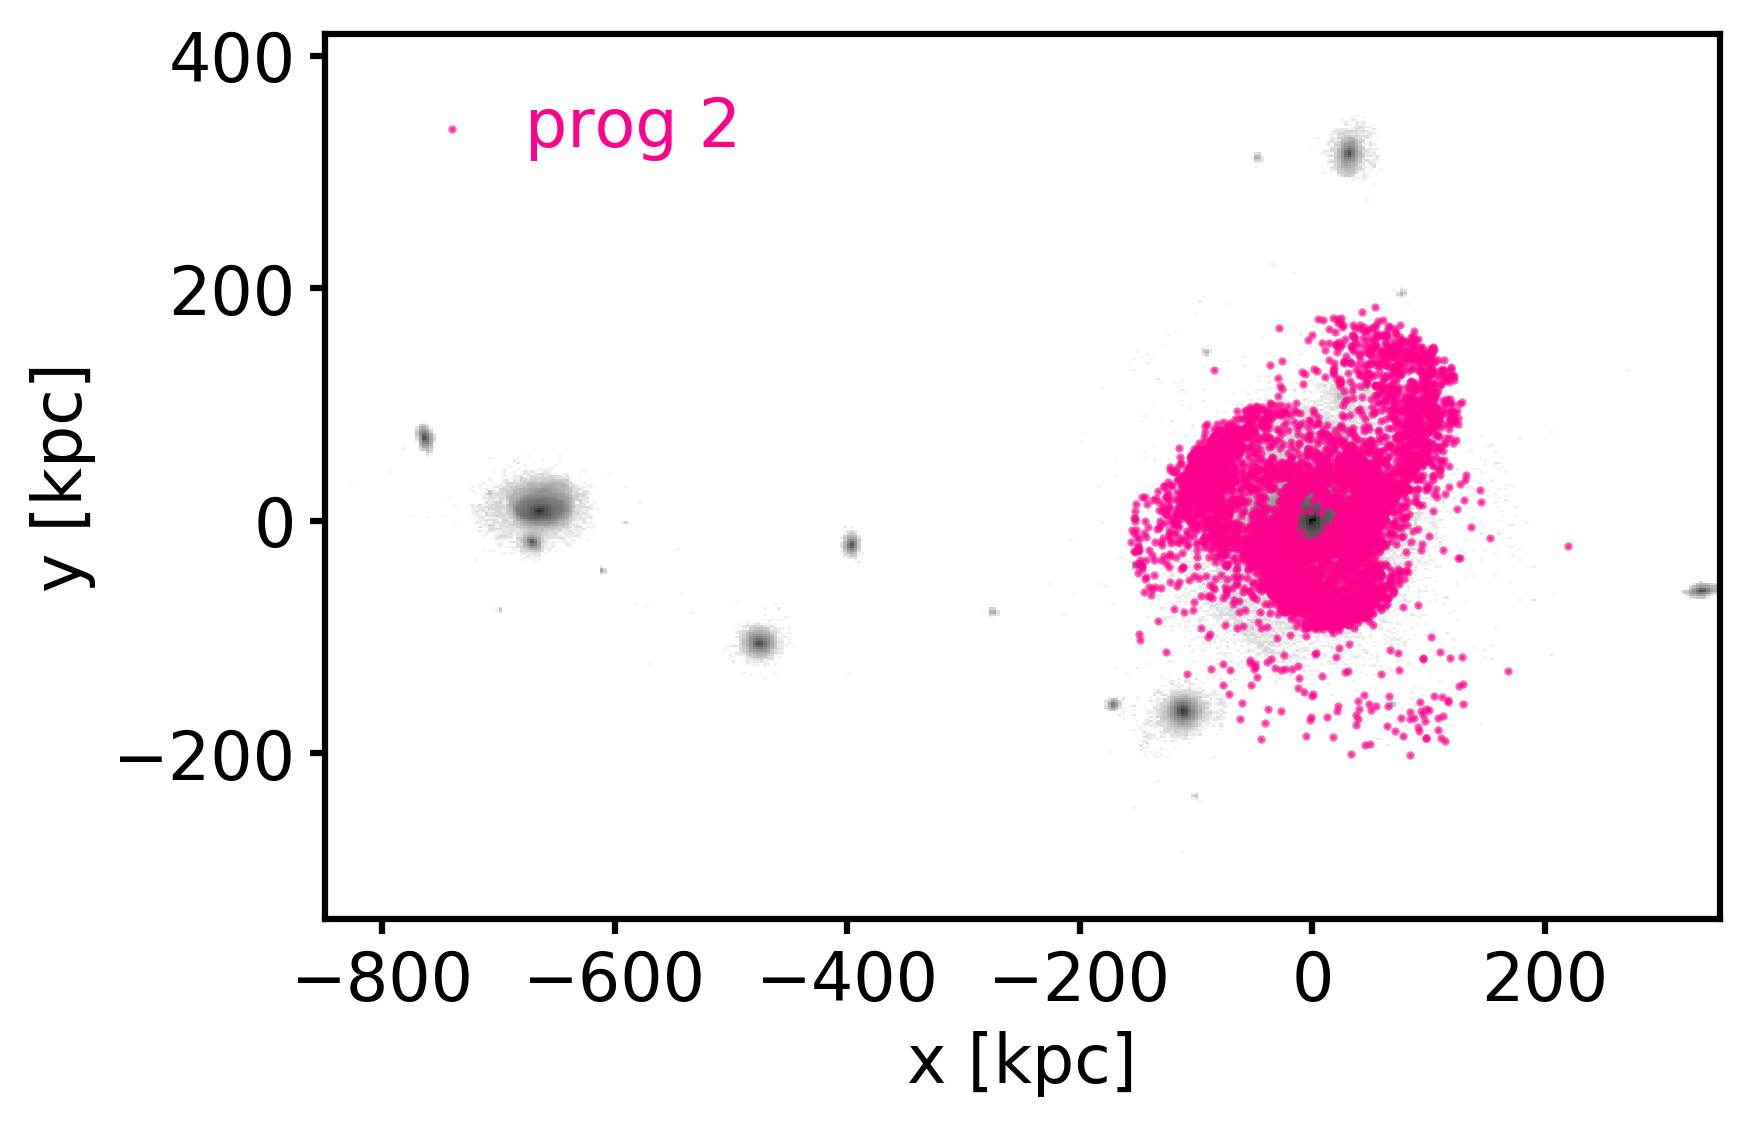
\includegraphics[width=\textwidth]{plots/Dynamics/dist/xy_dist_selected_GCs_prog_2_snap_127.png}
    	\label{fig:prog2_xy}
    \end{subfigure}
    ~ %add desired spacing between images, e. g. ~, \quad, \qquad, \hfill etc. 
    %(or a blank line to force the subfigure onto a new line)
    \begin{subfigure}[c]{0.45\textwidth}
        \centering
    	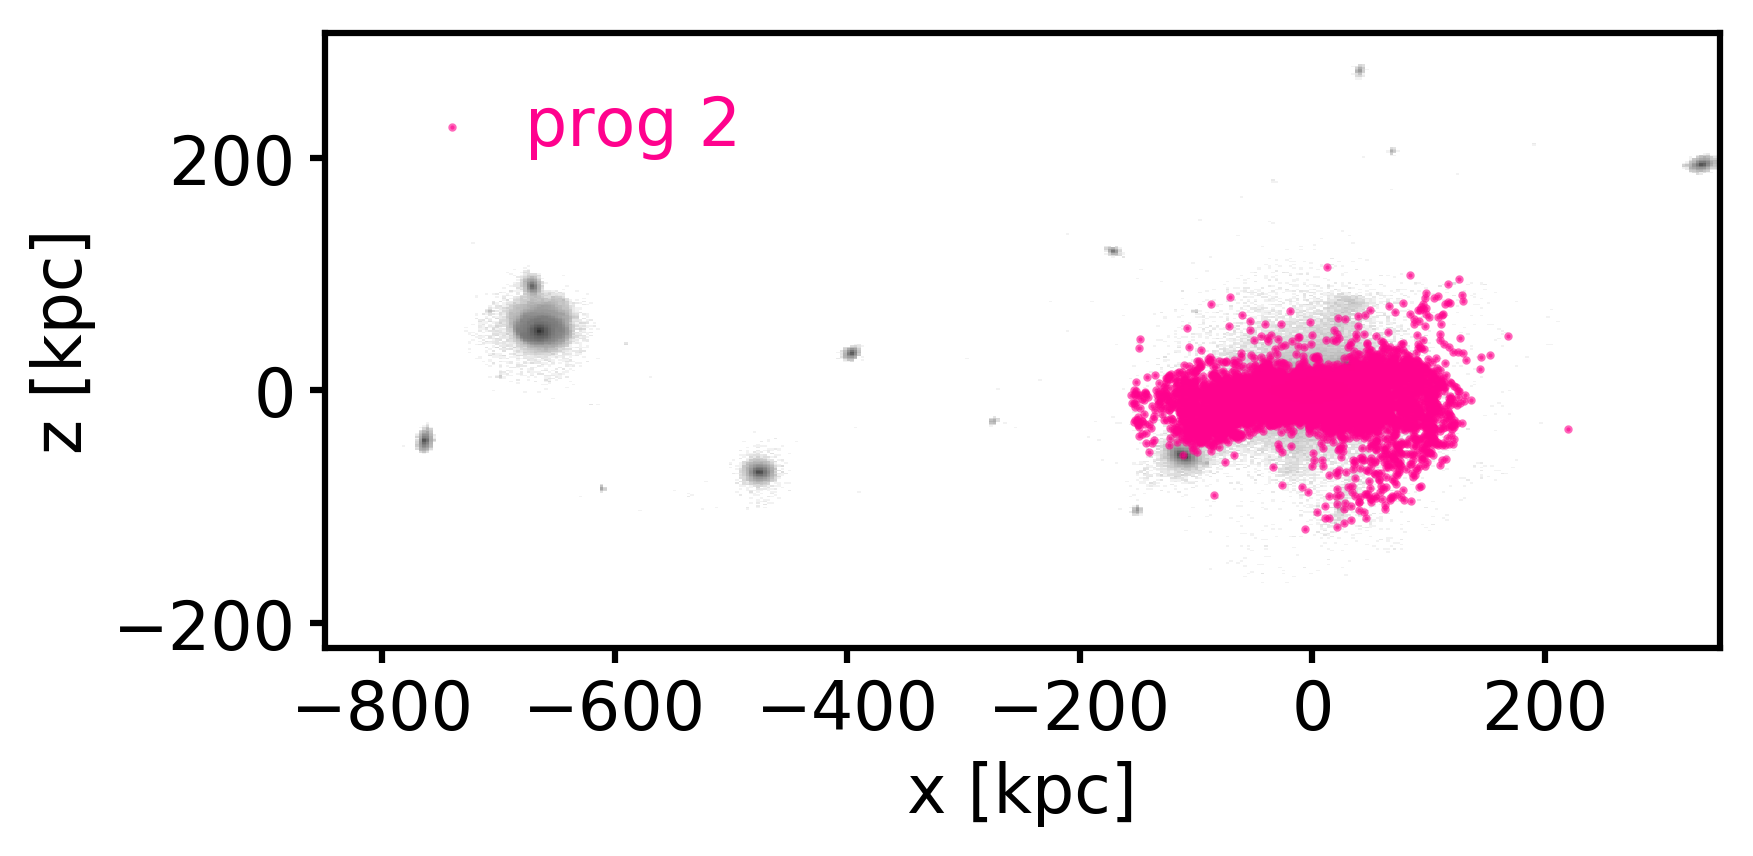
\includegraphics[width=\textwidth]{plots/Dynamics/dist/xz_dist_selected_GCs_prog_2_snap_127.png}
	    \label{fig:prog2_xz}
    \end{subfigure}
    
    \begin{subfigure}[c]{0.45\textwidth}
    \centering
    	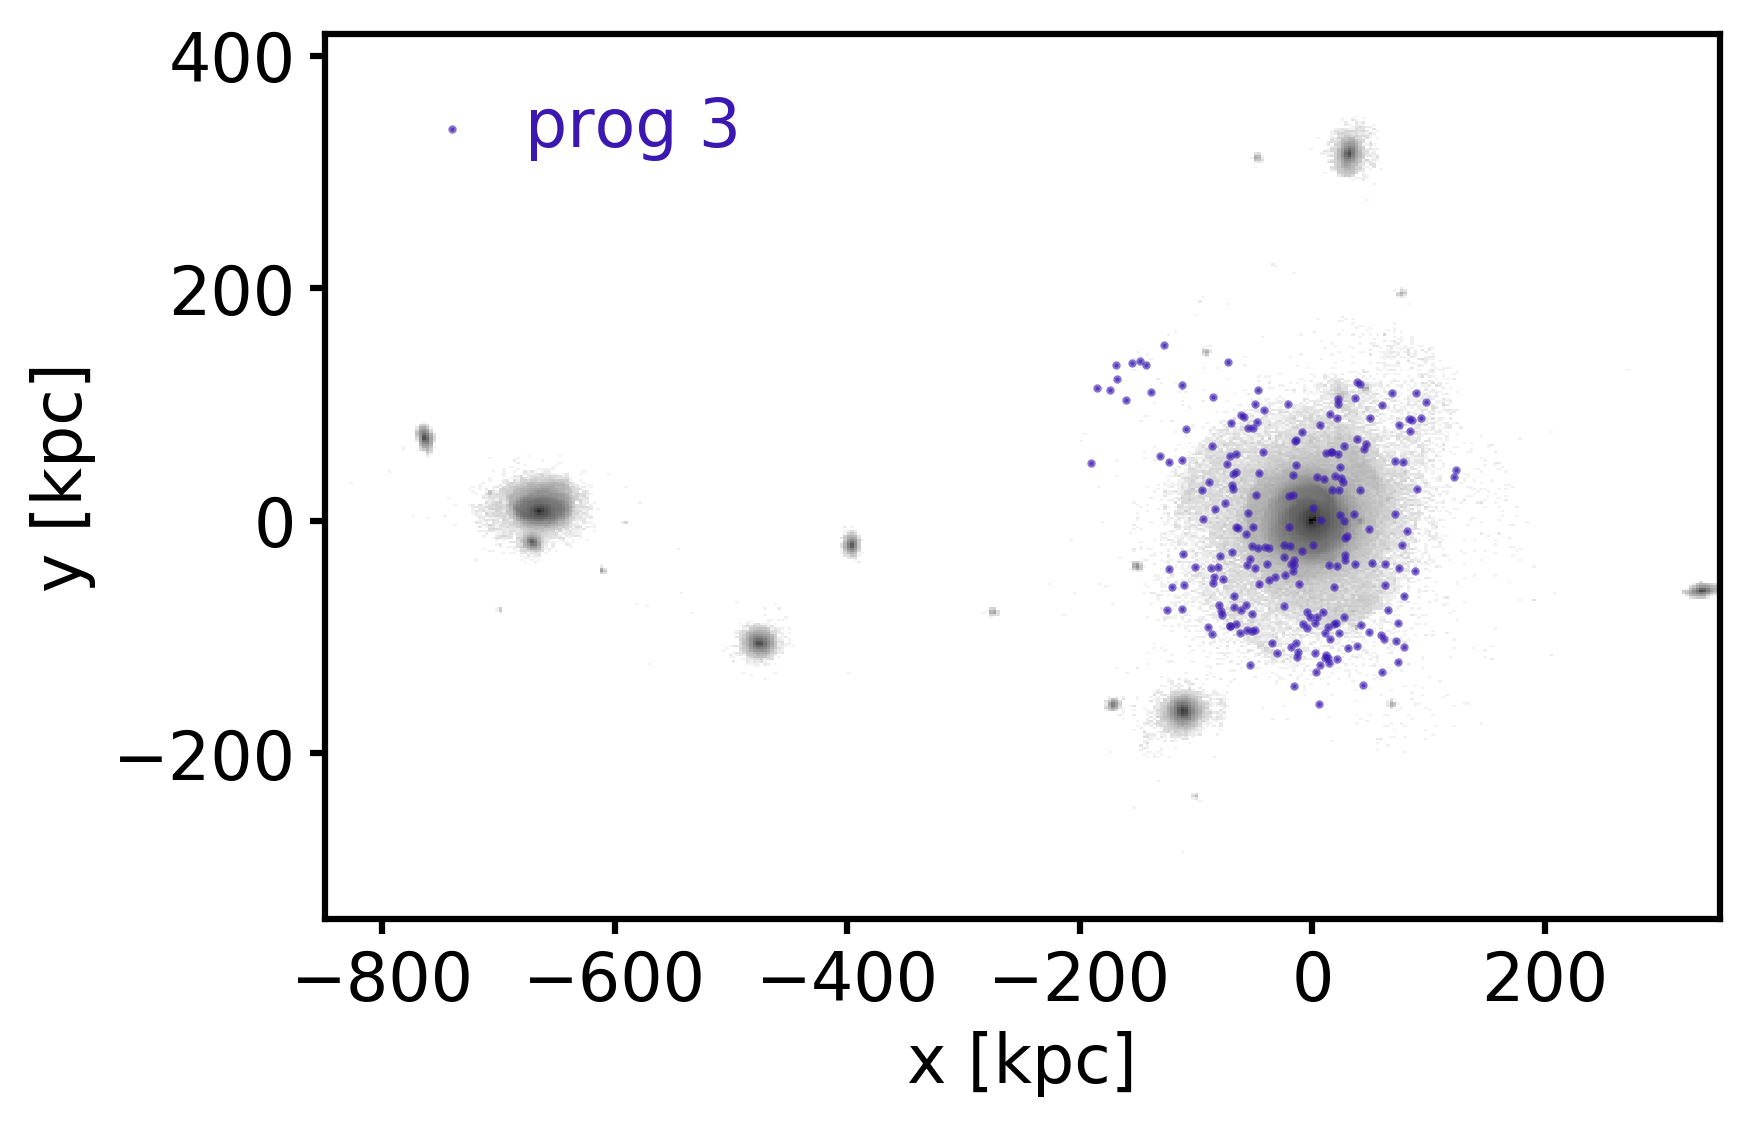
\includegraphics[width=\textwidth]{plots/Dynamics/dist/xy_dist_selected_GCs_prog_3_snap_127.png}
    	\label{fig:prog3_xy}
    \end{subfigure}
    ~ %add desired spacing between images, e. g. ~, \quad, \qquad, \hfill etc. 
    %(or a blank line to force the subfigure onto a new line)
    \begin{subfigure}[c]{0.45\textwidth}
        \centering
    	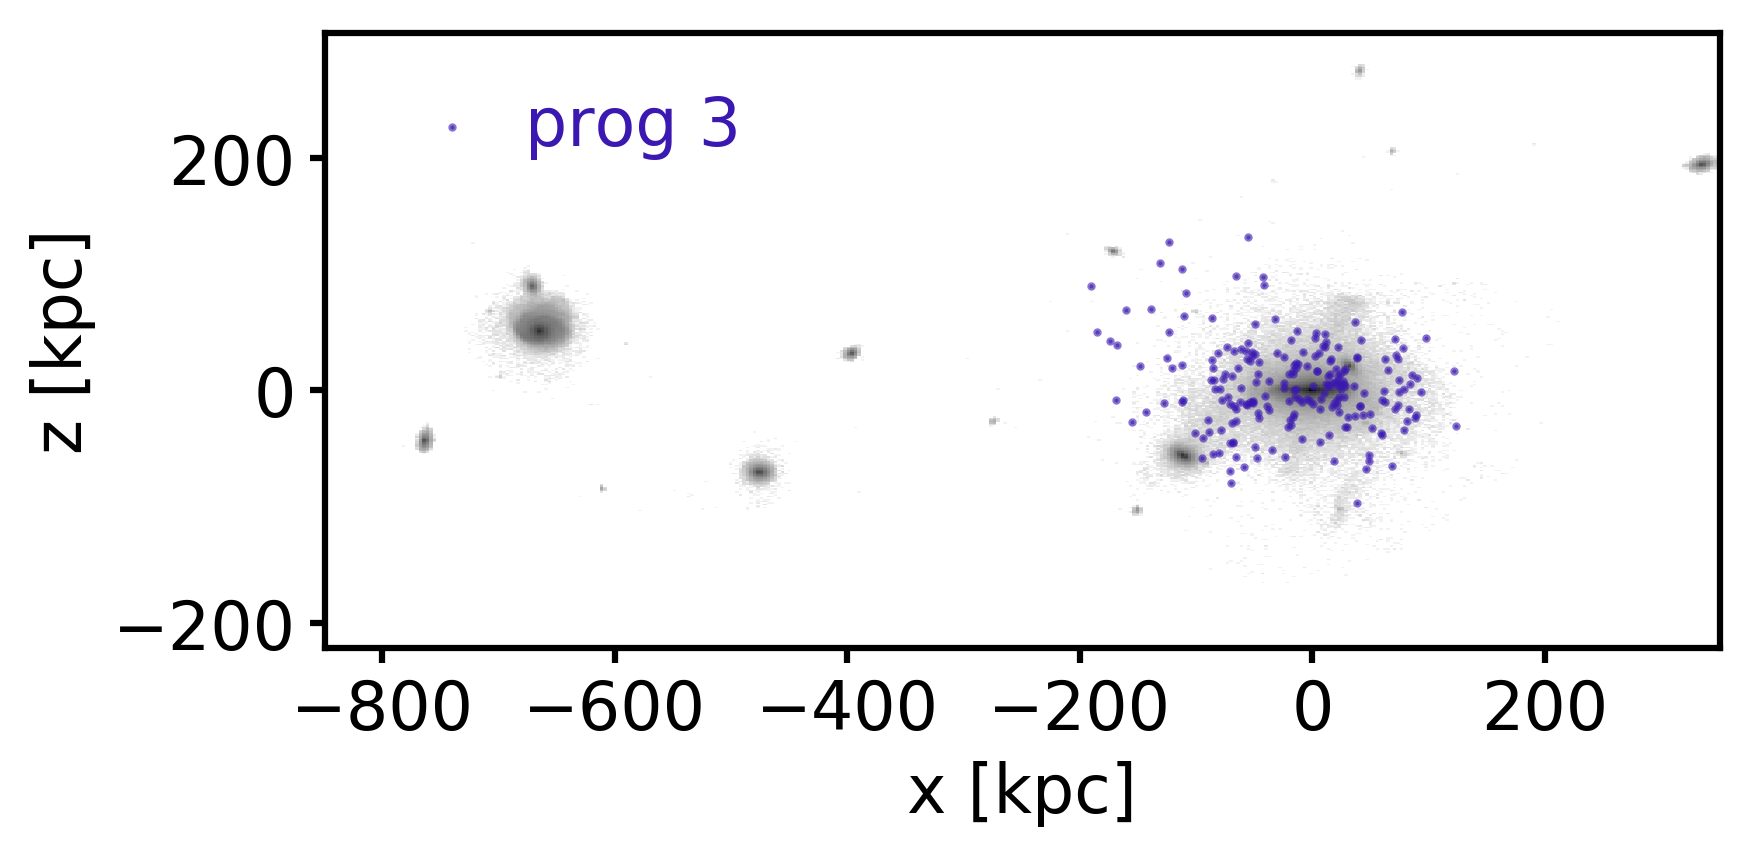
\includegraphics[width=\textwidth]{plots/Dynamics/dist/xz_dist_selected_GCs_prog_3_snap_127.png}
	    \label{fig:prog3_xz}
    \end{subfigure}
    
    \begin{subfigure}[c]{0.45\textwidth}
    \centering
    	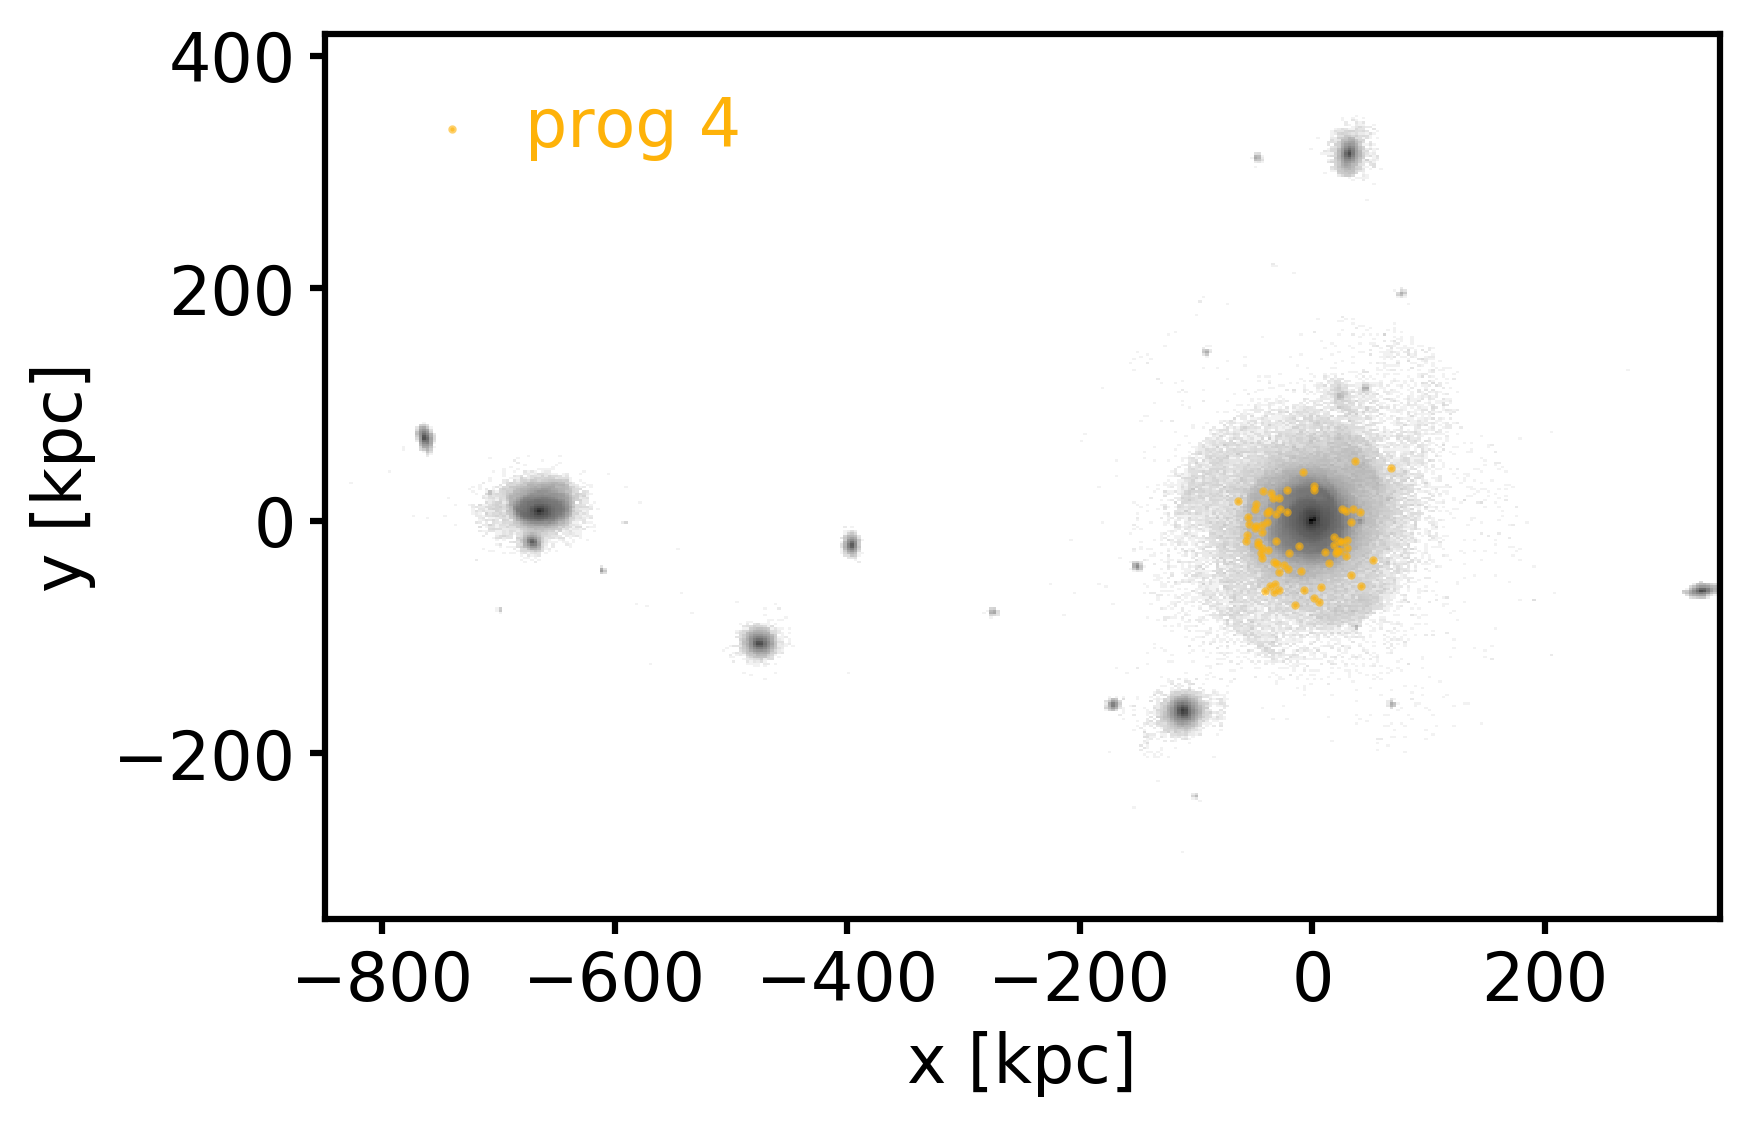
\includegraphics[width=\textwidth]{plots/Dynamics/dist/xy_dist_selected_GCs_prog_4_snap_127.png}
    	\label{fig:prog4_xy}
    \end{subfigure}
    ~ %add desired spacing between images, e. g. ~, \quad, \qquad, \hfill etc. 
    %(or a blank line to force the subfigure onto a new line)
    \begin{subfigure}[c]{0.45\textwidth}
        \centering
    	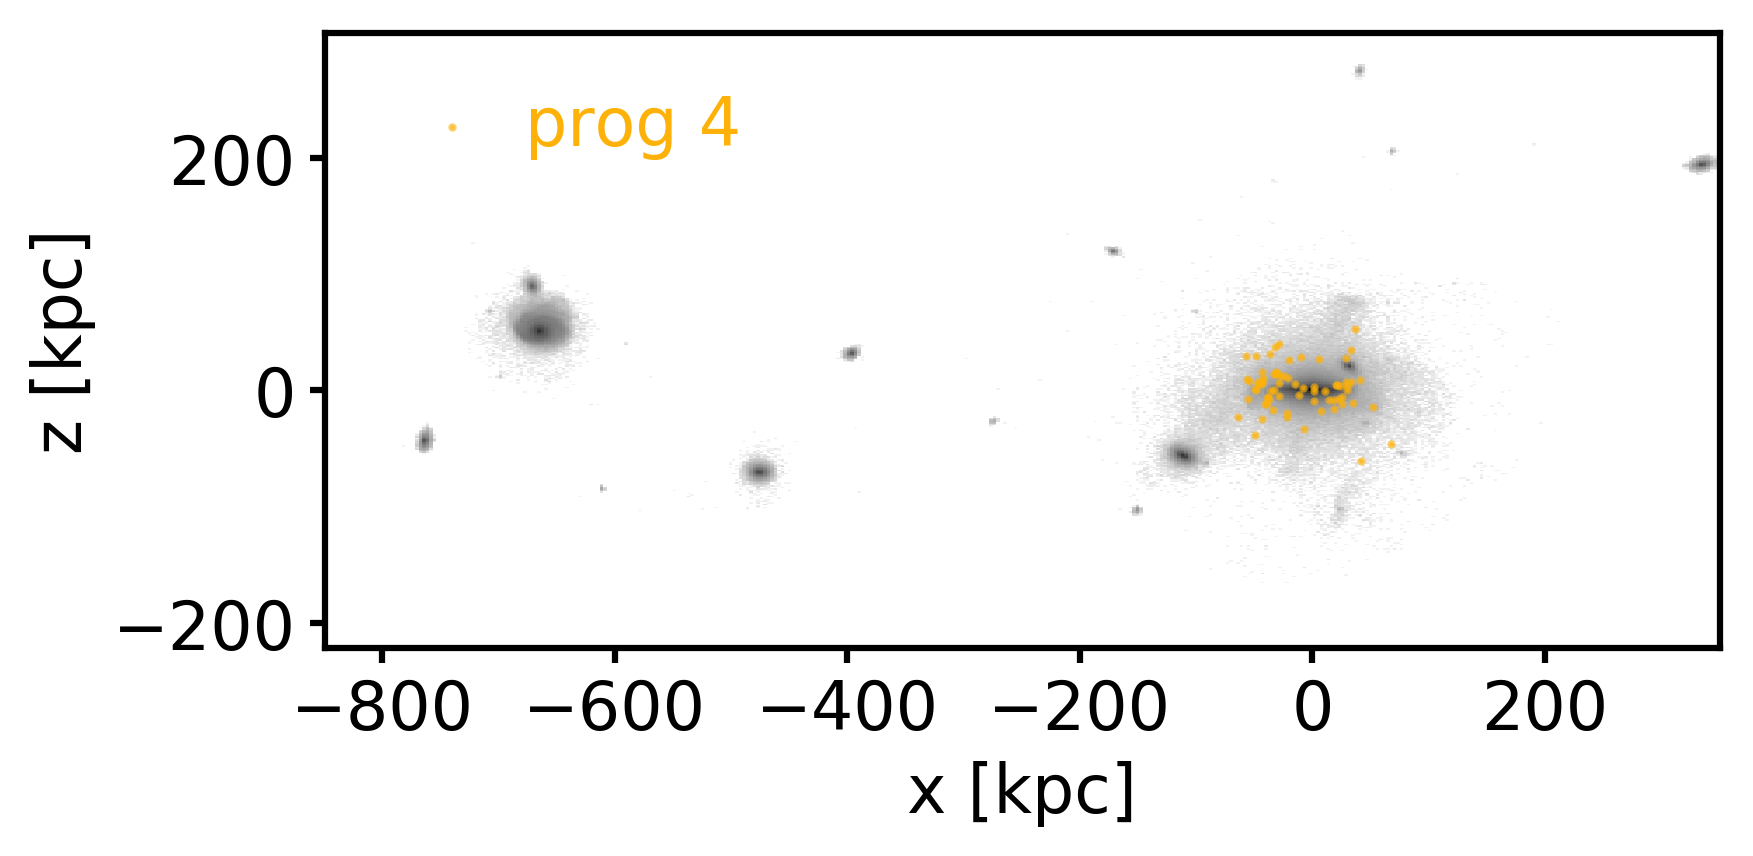
\includegraphics[width=\textwidth]{plots/Dynamics/dist/xz_dist_selected_GCs_prog_4_snap_127.png}
	    \label{fig:prog4_xz}
    \end{subfigure}
    \caption{.}\label{fig:progenitors_distribution}
\end{figure}


\subsection{Globular clusters in action space}\label{subsec:GCs_action_space}
Now, we look at the \ac{GC} distribution in action space. Our assumption is that in the "true" potential, \acp{GC} are very clumped since they should retain dynamical memory from their former \ac{DG} and therefore their \ac{DF} should be a delta function. In section \ref{subsubsec:GCs_actions_right_pot}, we will look at the distribution in the fitted potential at redshift 0. In section \ref{subsubsec:GCs_actions_varying_pot}, we evaluate actions in varying potentials to test our assumption of \acp{GC} being most clumped in action space in the "true" potential. 

\subsubsection{Best fit potential}\label{subsubsec:GCs_actions_right_pot}

\begin{figure}[htbp]
    \centering
    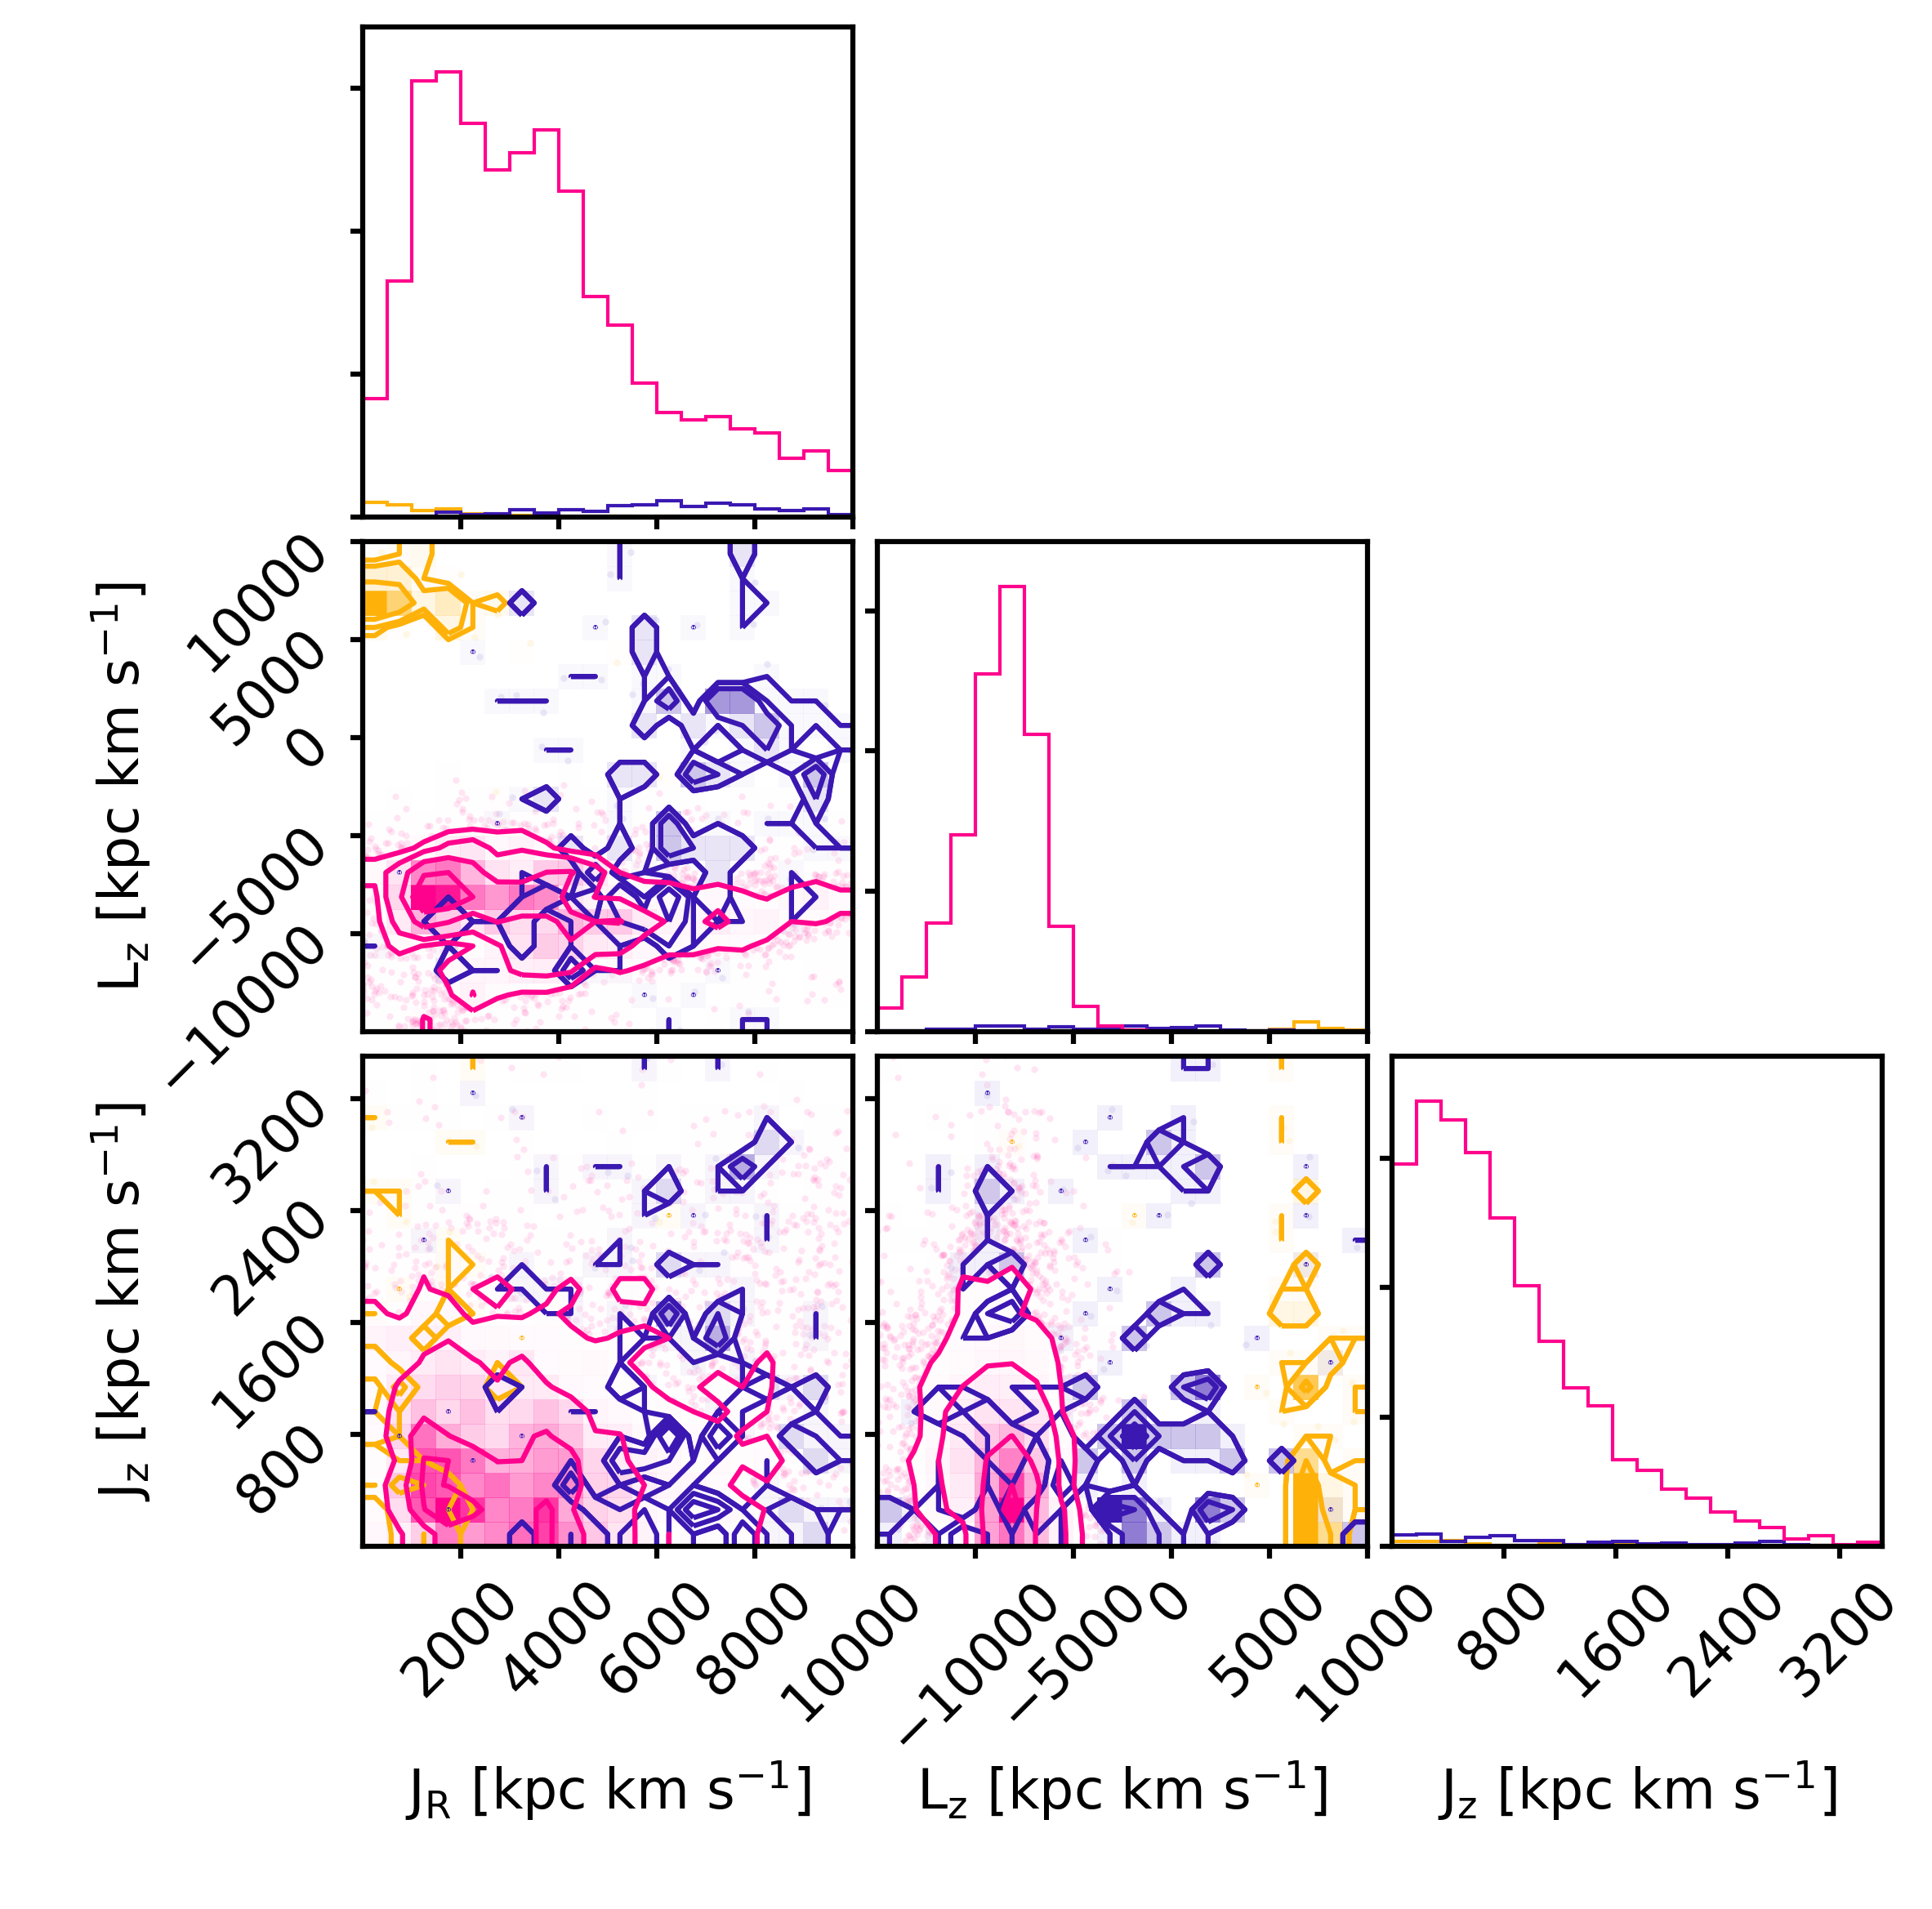
\includegraphics[width=1.0\textwidth]{plots/Dynamics/prog234_actions_snap_127.png}
    \caption{Selected \acp{GC} from three different \acp{DG} in action space.}
    \label{fig:act_both_merg_best_pot}
\end{figure}



\subsubsection{Varying potentials}\label{subsubsec:GCs_actions_varying_pot}

\begin{figure}[htbp]
    \centering
	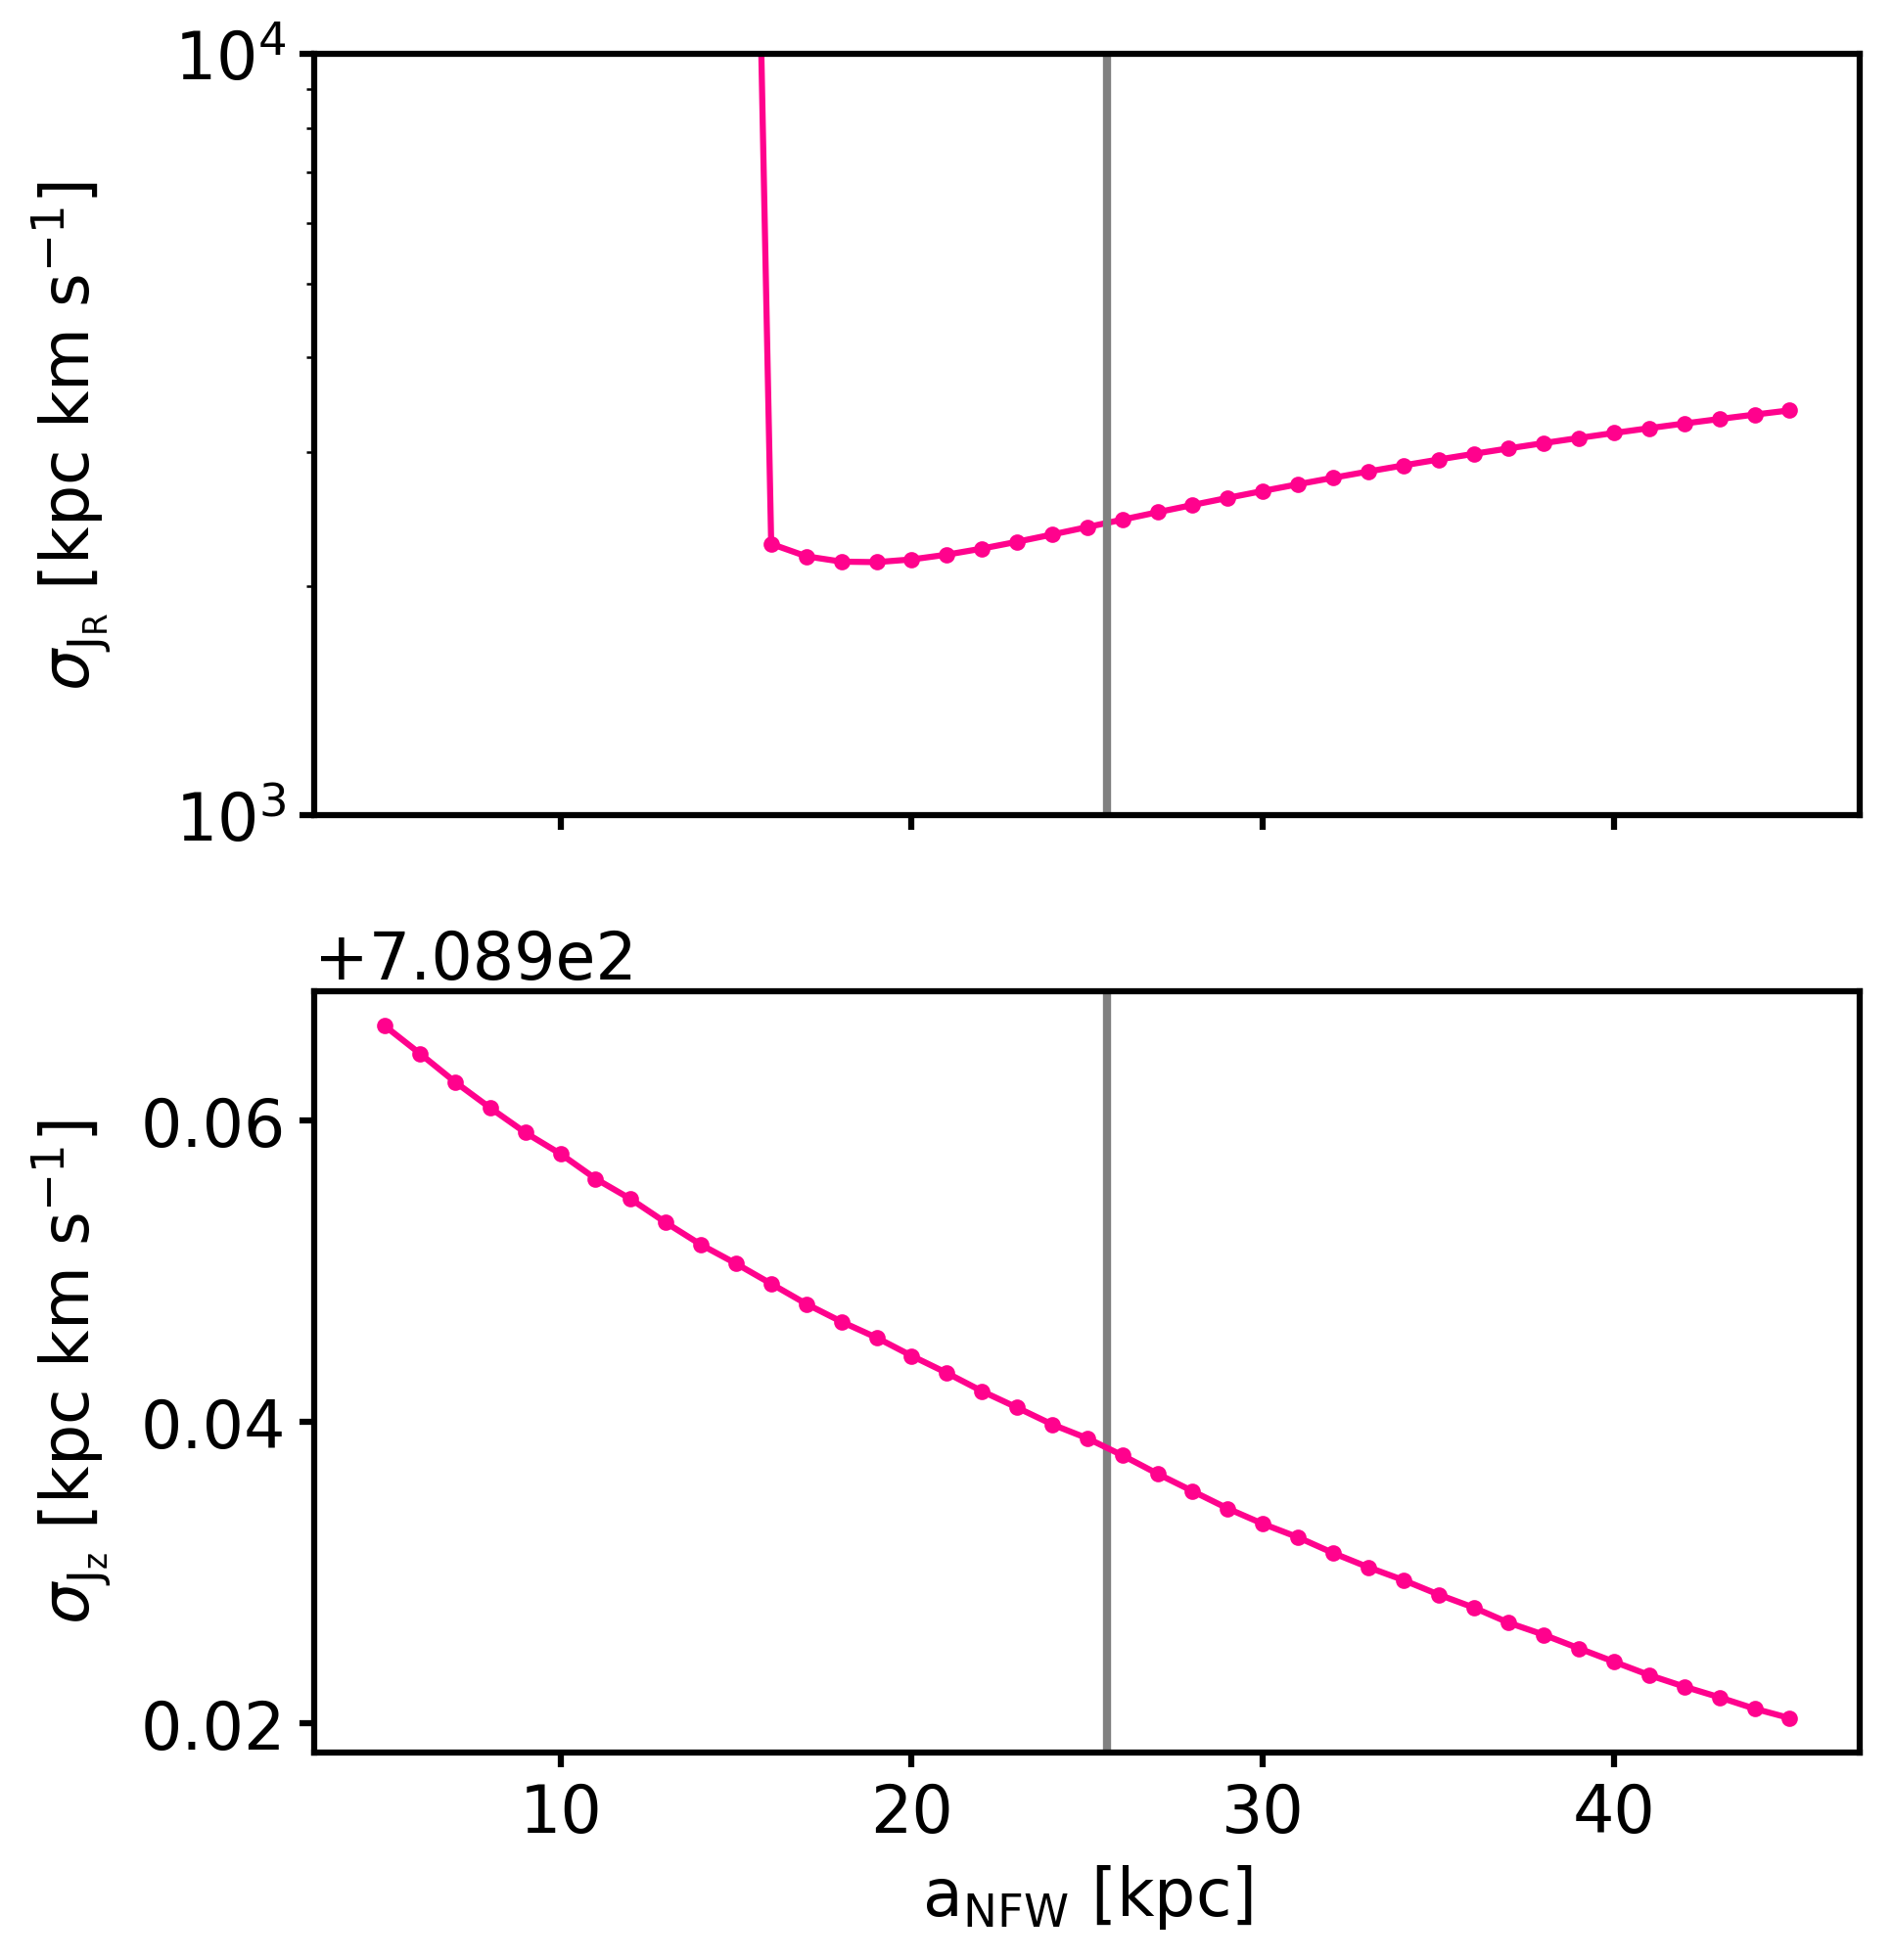
\includegraphics[width=0.6\textwidth]{plots/Dynamics/prog2/a_NFW_diagnostic_plot_std_prog2_all.png}
	\label{fig:NFW_diag_prog2}
\caption{.}
\end{figure}

\begin{figure}[b]
    \centering
	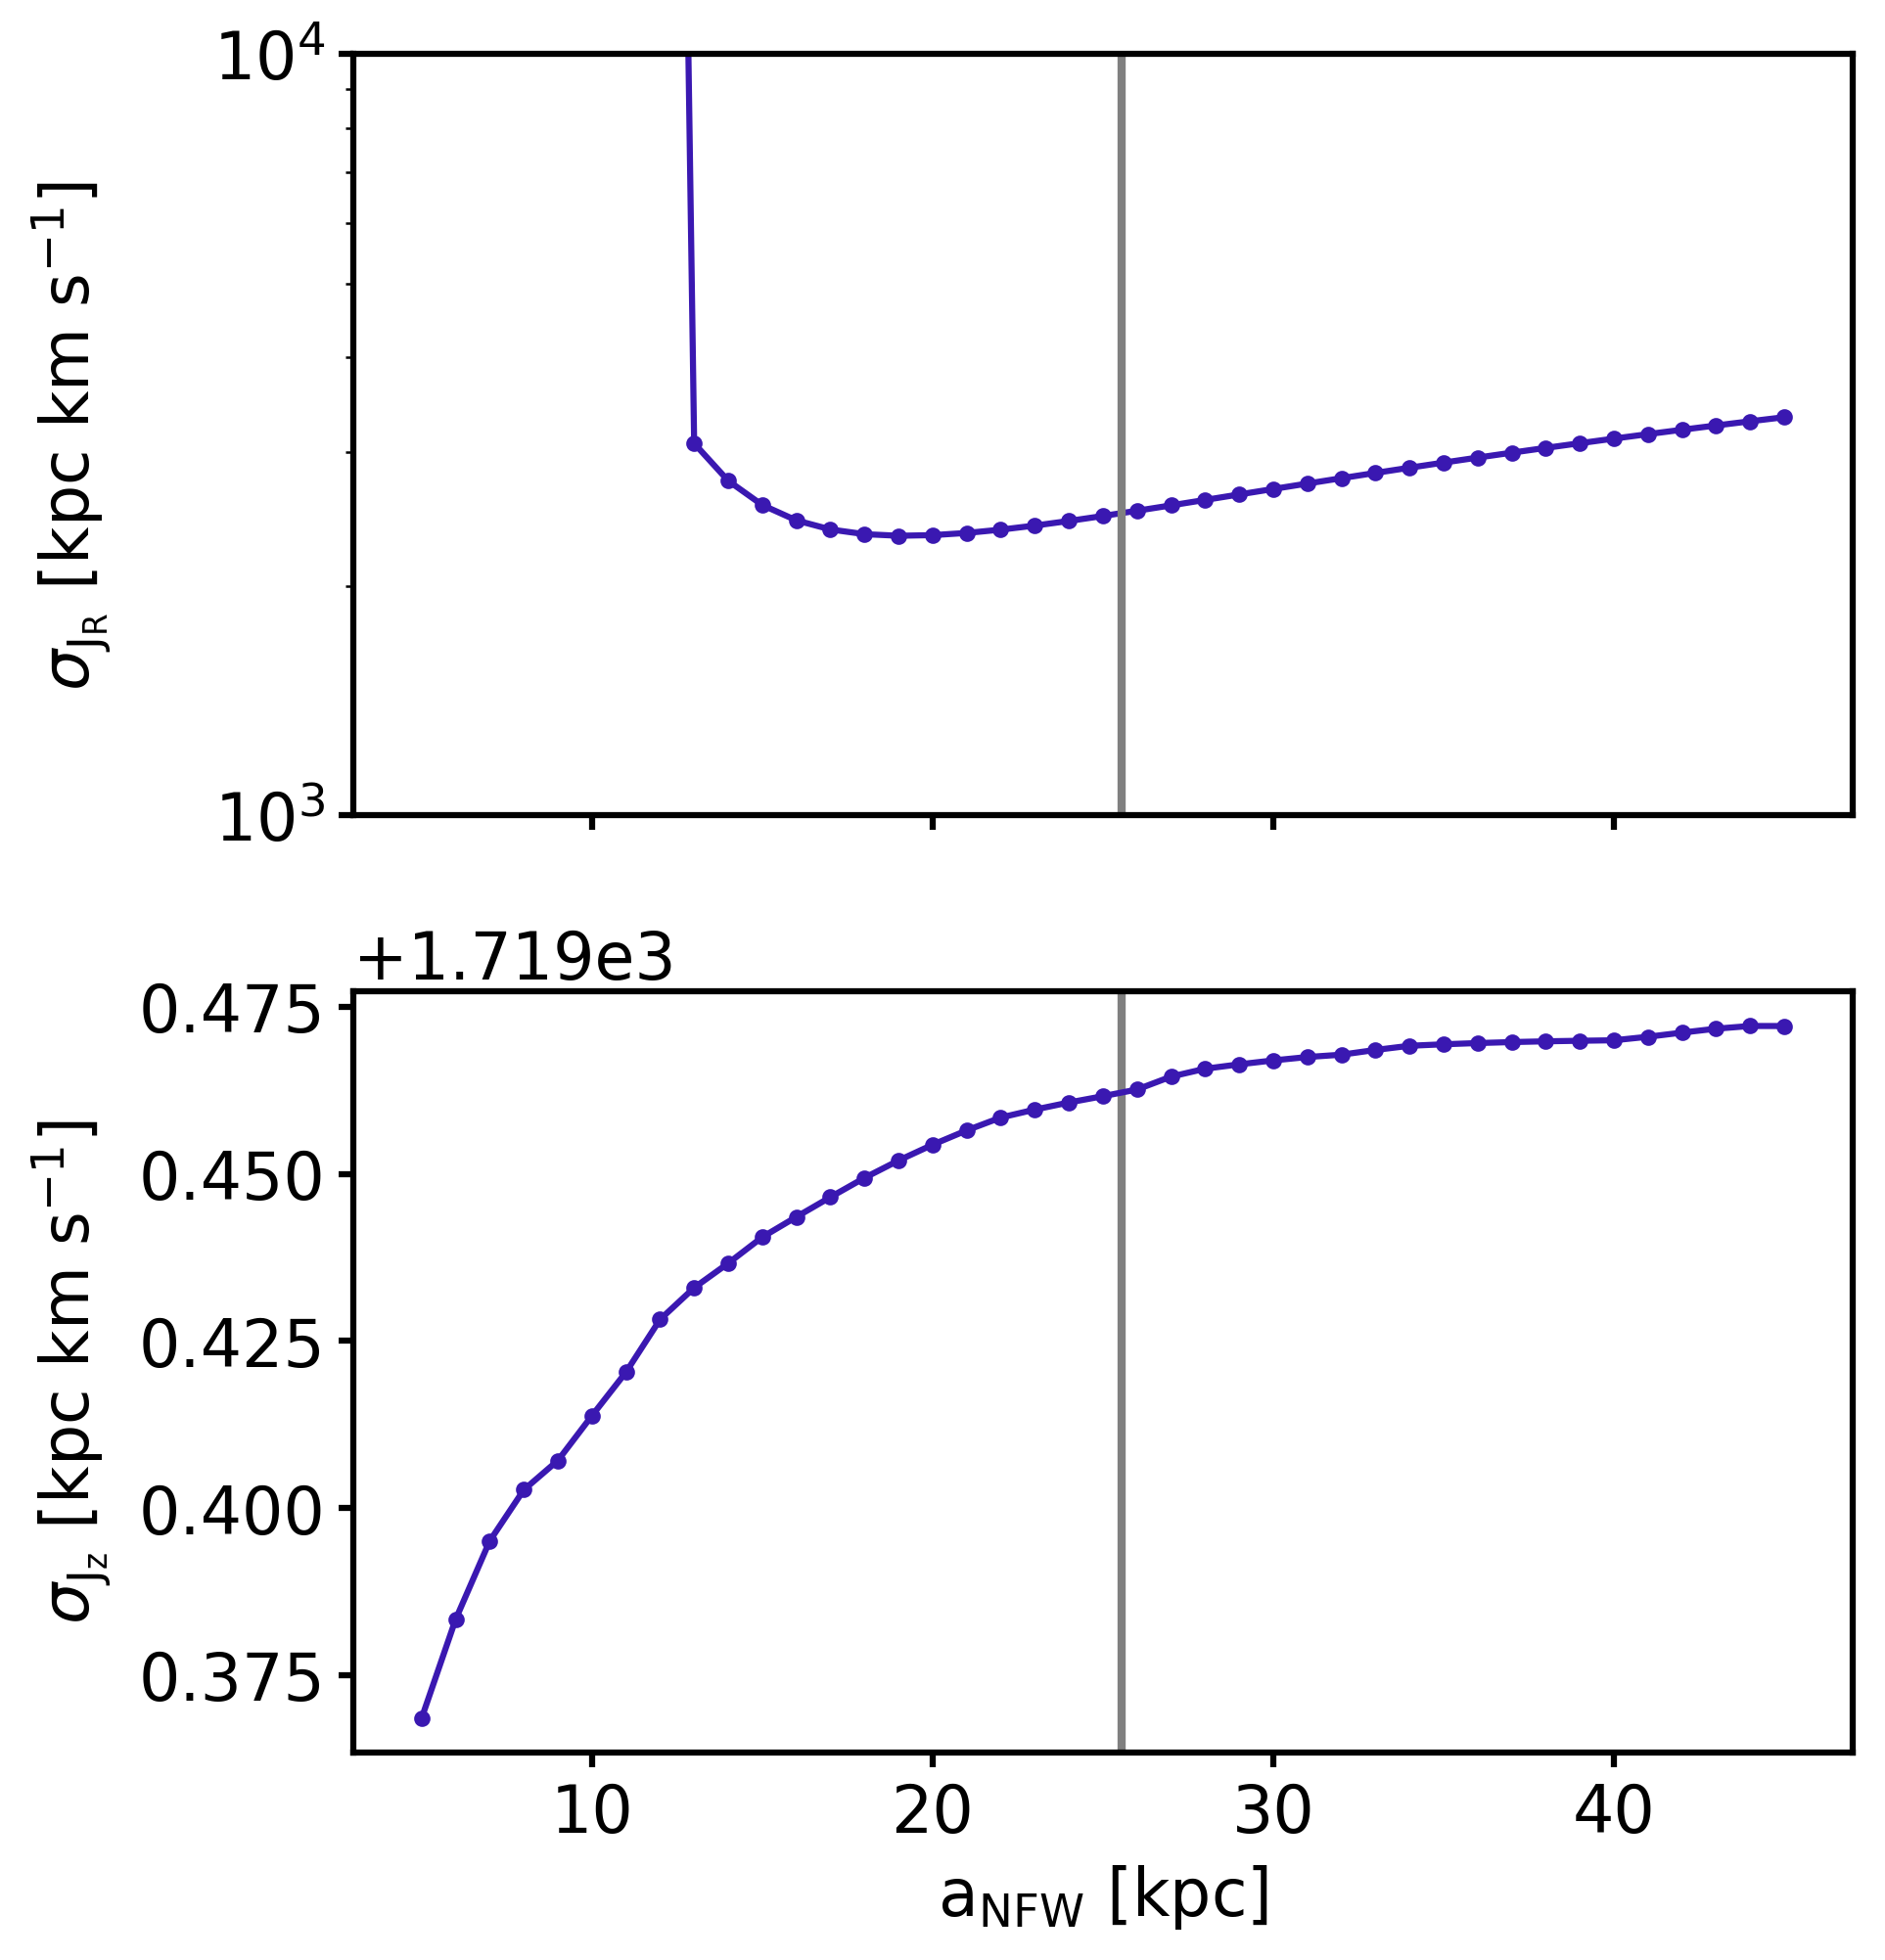
\includegraphics[width=0.6\textwidth]{plots/Dynamics/prog3/a_NFW_diagnostic_plot_std_prog3_all.png}
    \label{fig:NFW_diag_prog3}
\caption{.}
\end{figure}
\begin{figure}[b]
    \centering
	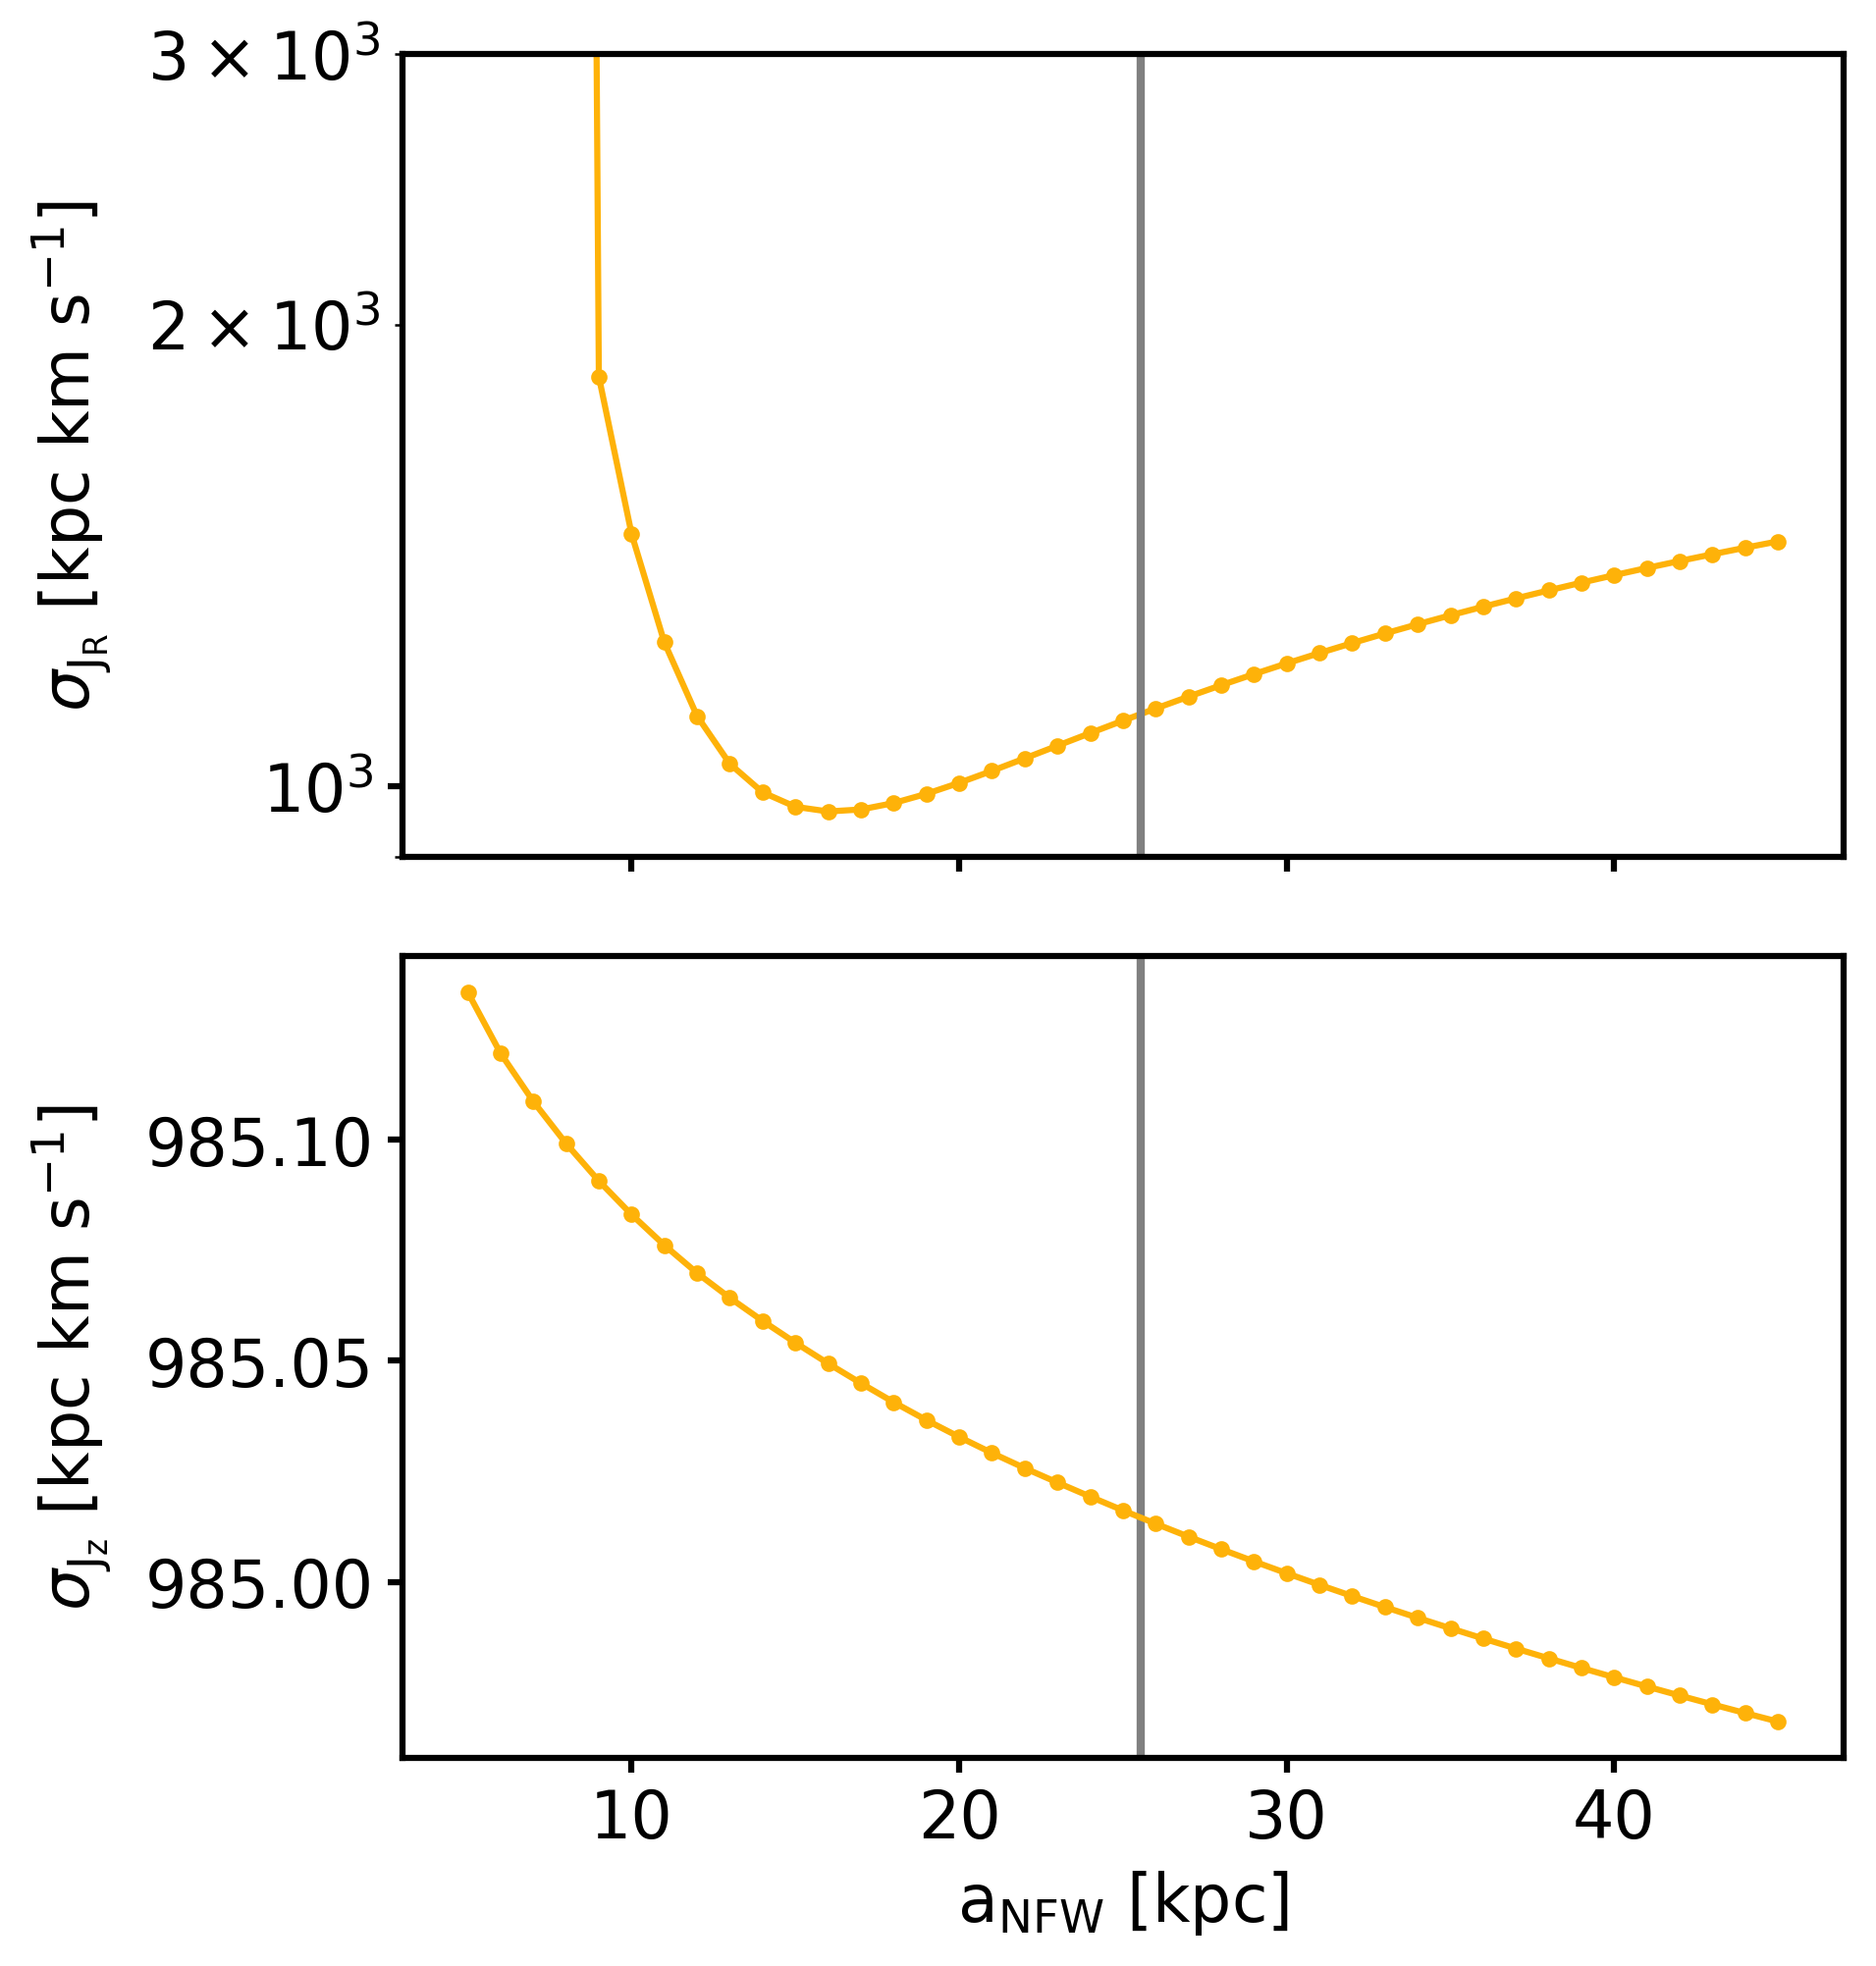
\includegraphics[width=0.6\textwidth]{plots/Dynamics/prog4/a_NFW_diagnostic_plot_std_prog4_all.png}
    \label{fig:NFW_diag_prog4}
\caption{.}
\end{figure}

\subsection{Time evolution of actions}\ref{subsec:}
We evaluate the time evolution of the orbits of the accreted \acp{GC} to how the actions evolved and to see if there was a point - probably shortly after their mergers - where the \acp{GC} were more clumped in action space. We calculate the actions of the selected particles in the best fit potential in each snapshot.  

\begin{figure}[htbp]
    \centering
	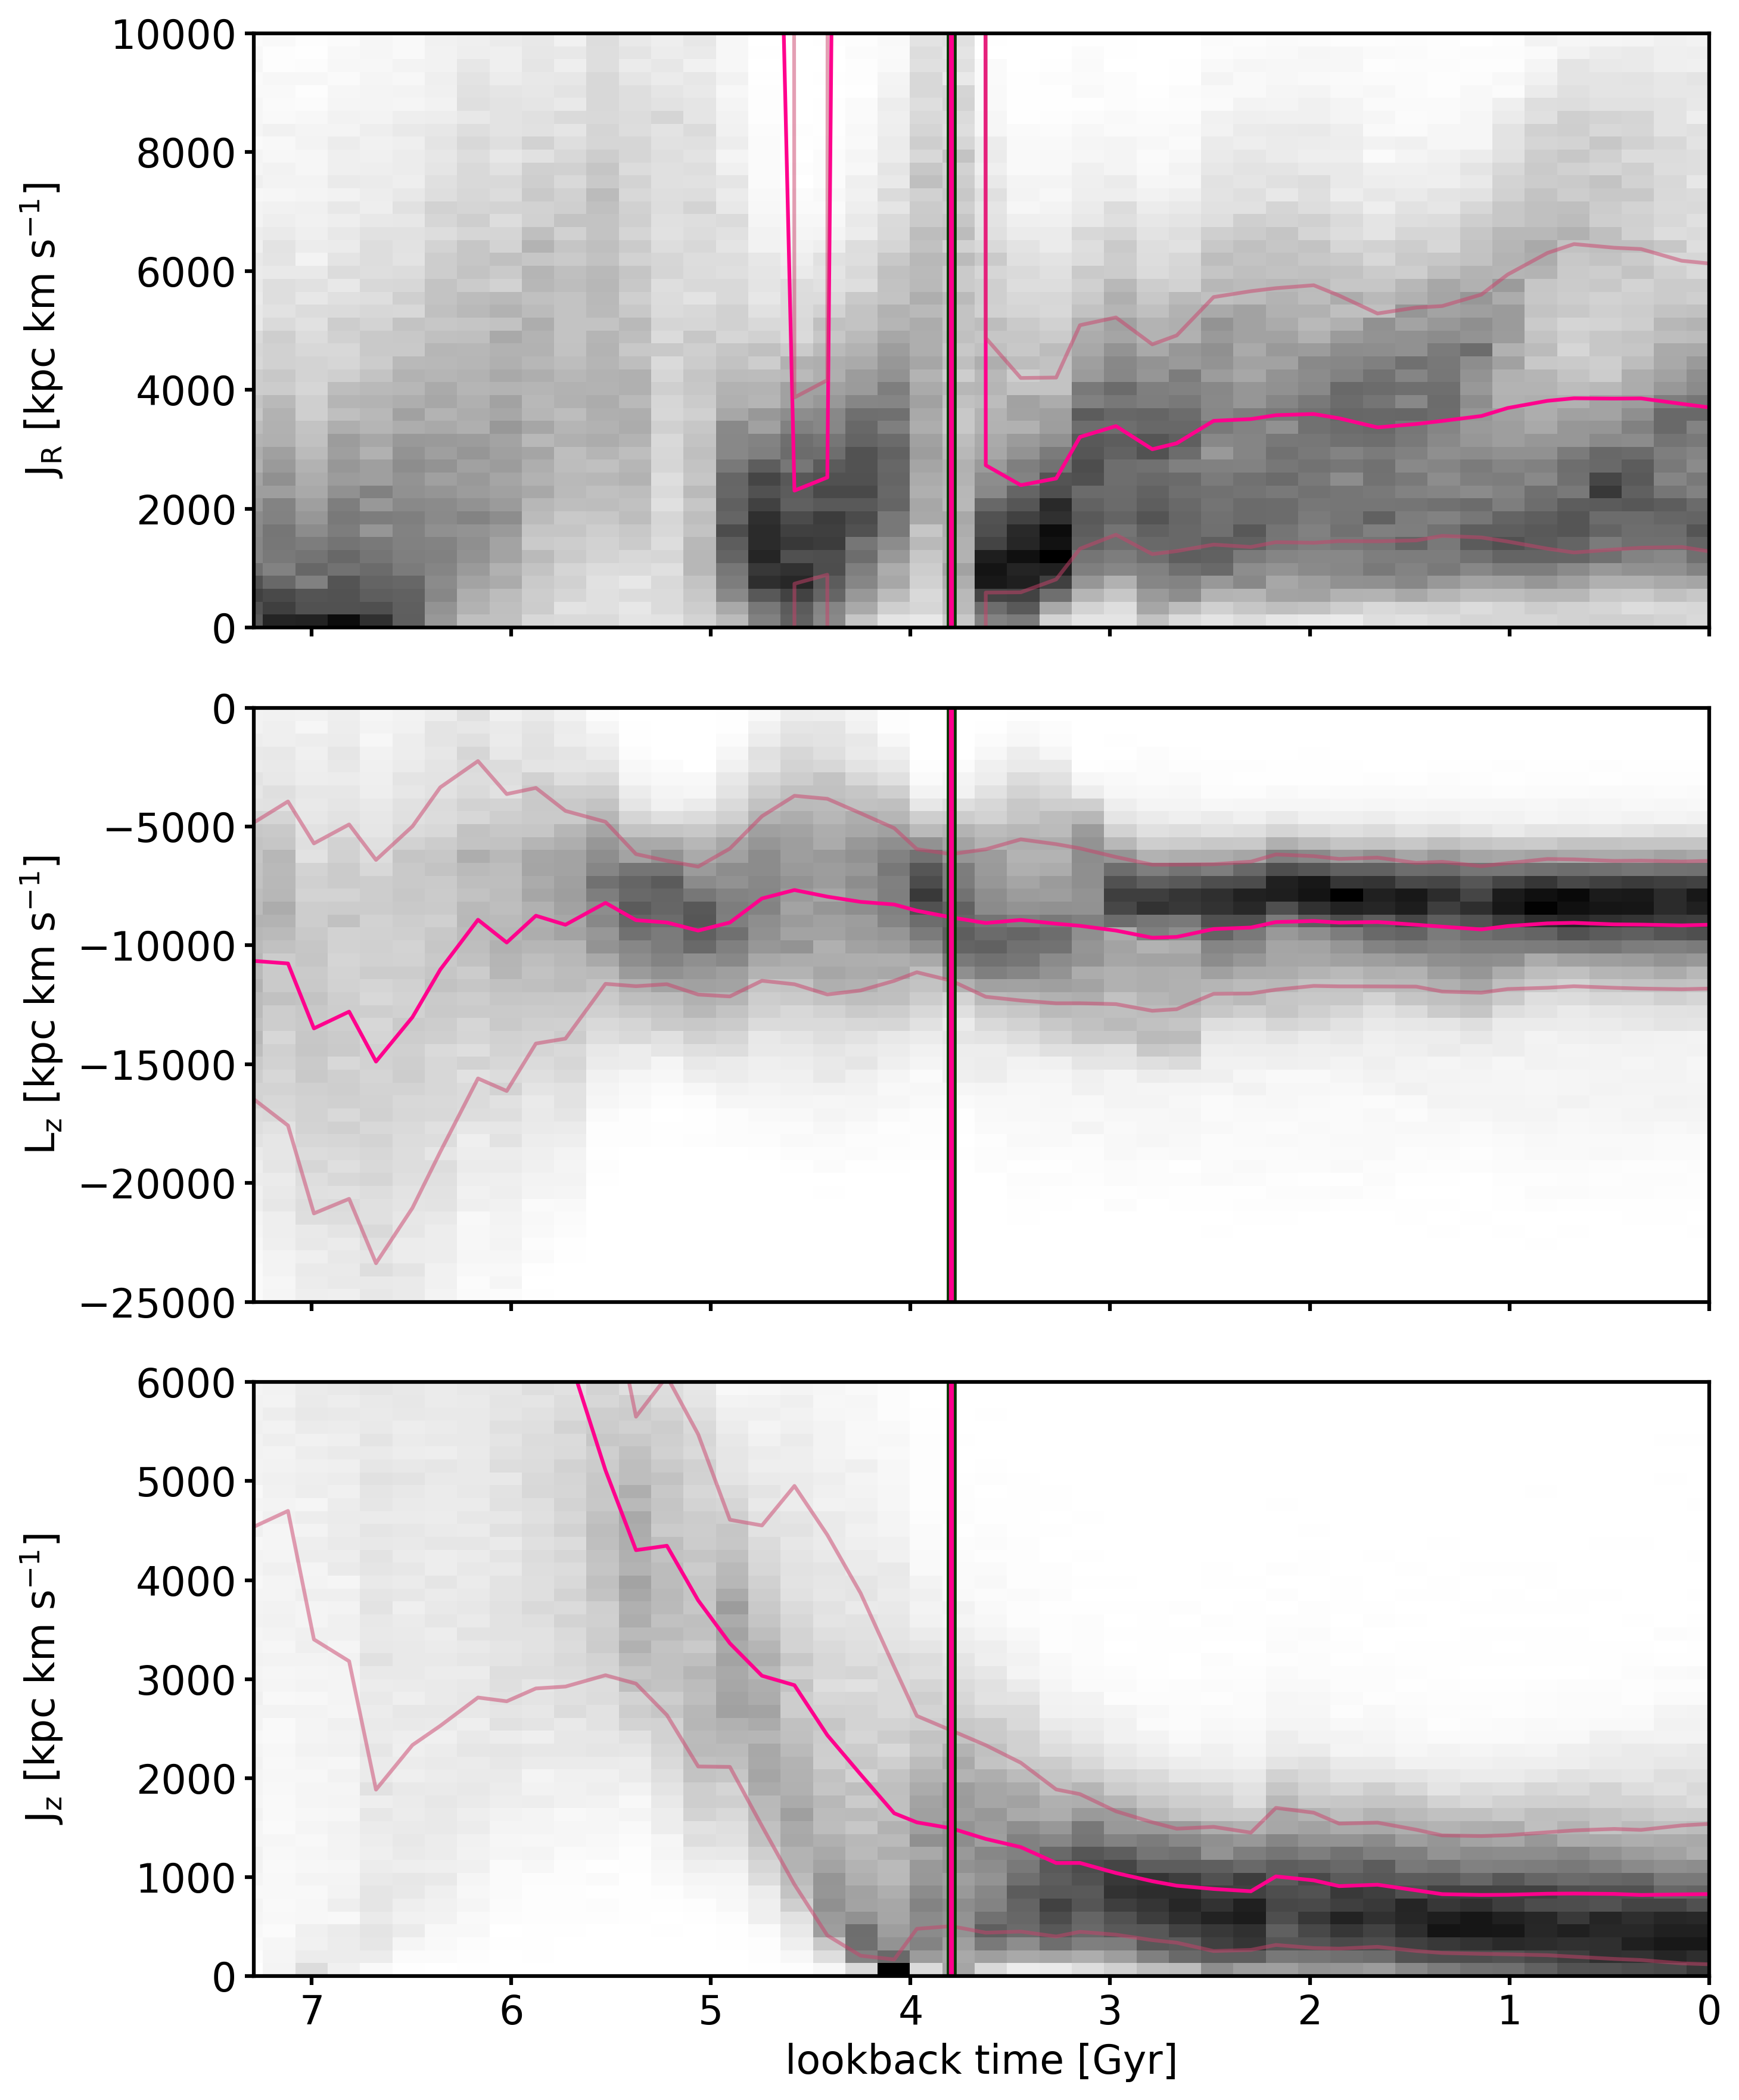
\includegraphics[width=\textwidth]{plots/Dynamics/prog2/action_time_evolution_hist_mean.png}
	\label{fig:time_ev_all_GCs}
	\caption{.}
\end{figure}
\begin{figure}
    \centering
	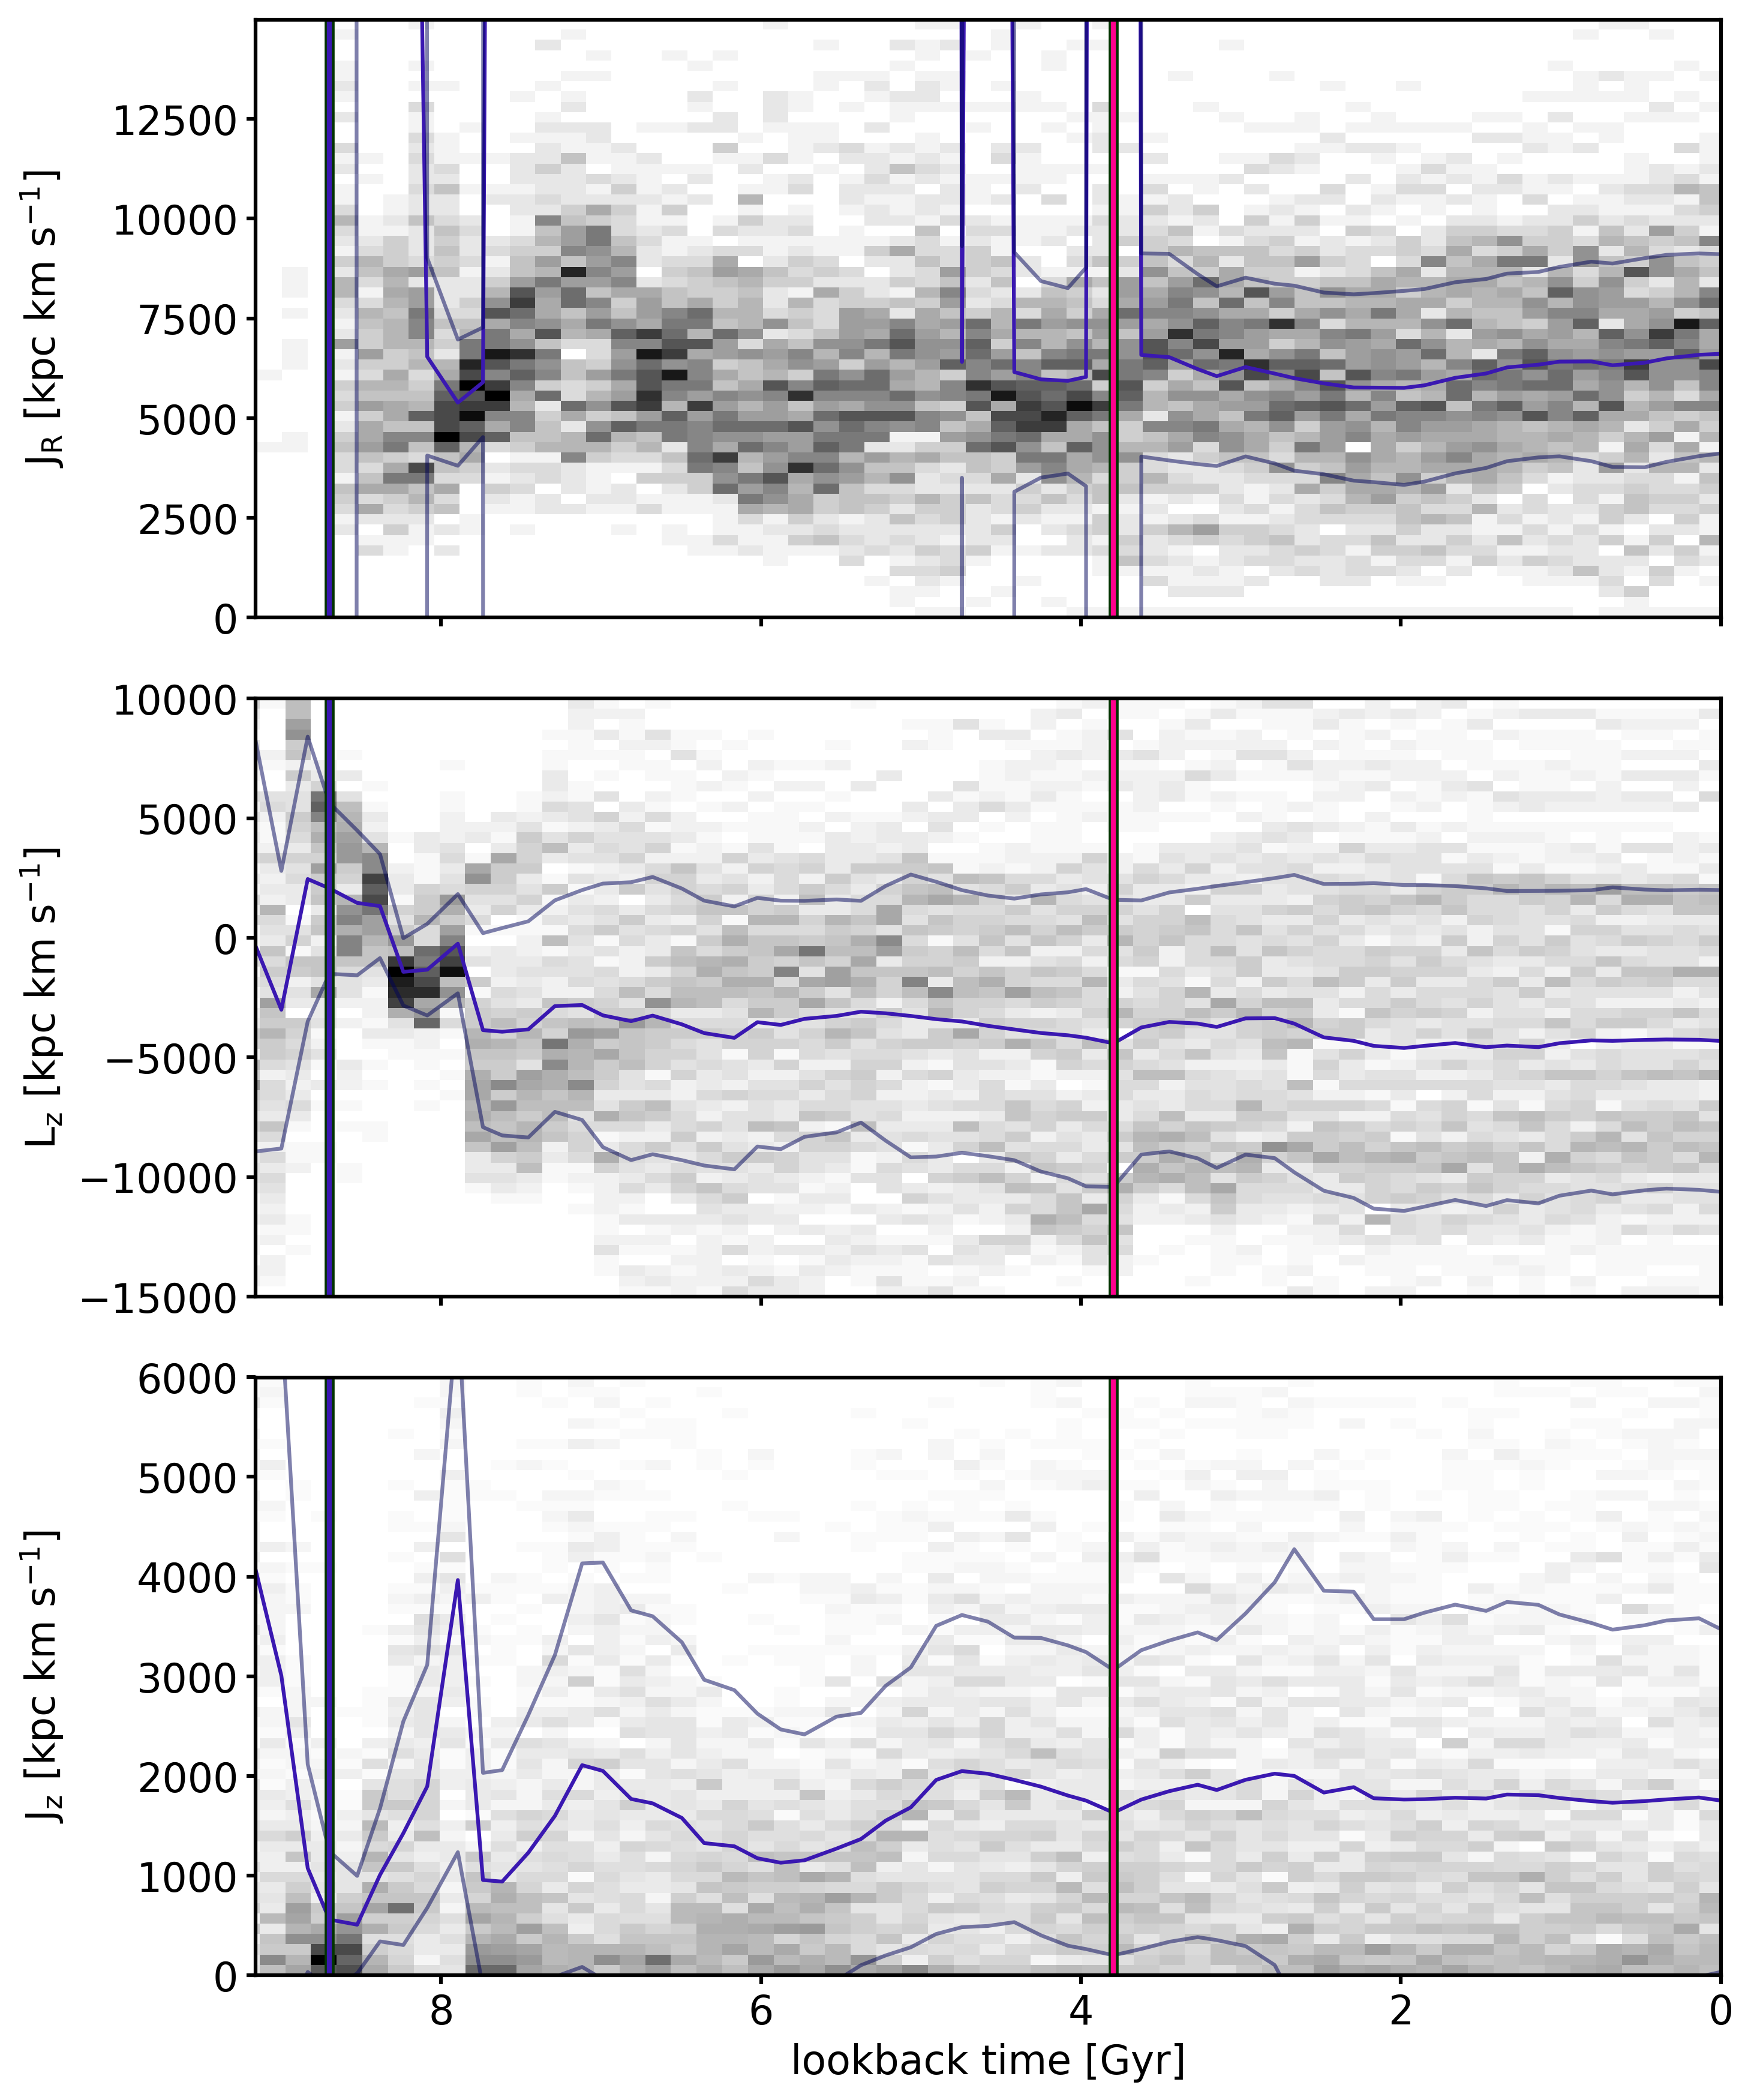
\includegraphics[width=\textwidth]{plots/Dynamics/prog3/action_time_evolution_hist_mean.png}
    \label{fig:time_ev_box_GCs}
    \caption{.}\label{fig:actions_time_evolution}
\end{figure}
\begin{figure}
    \centering
	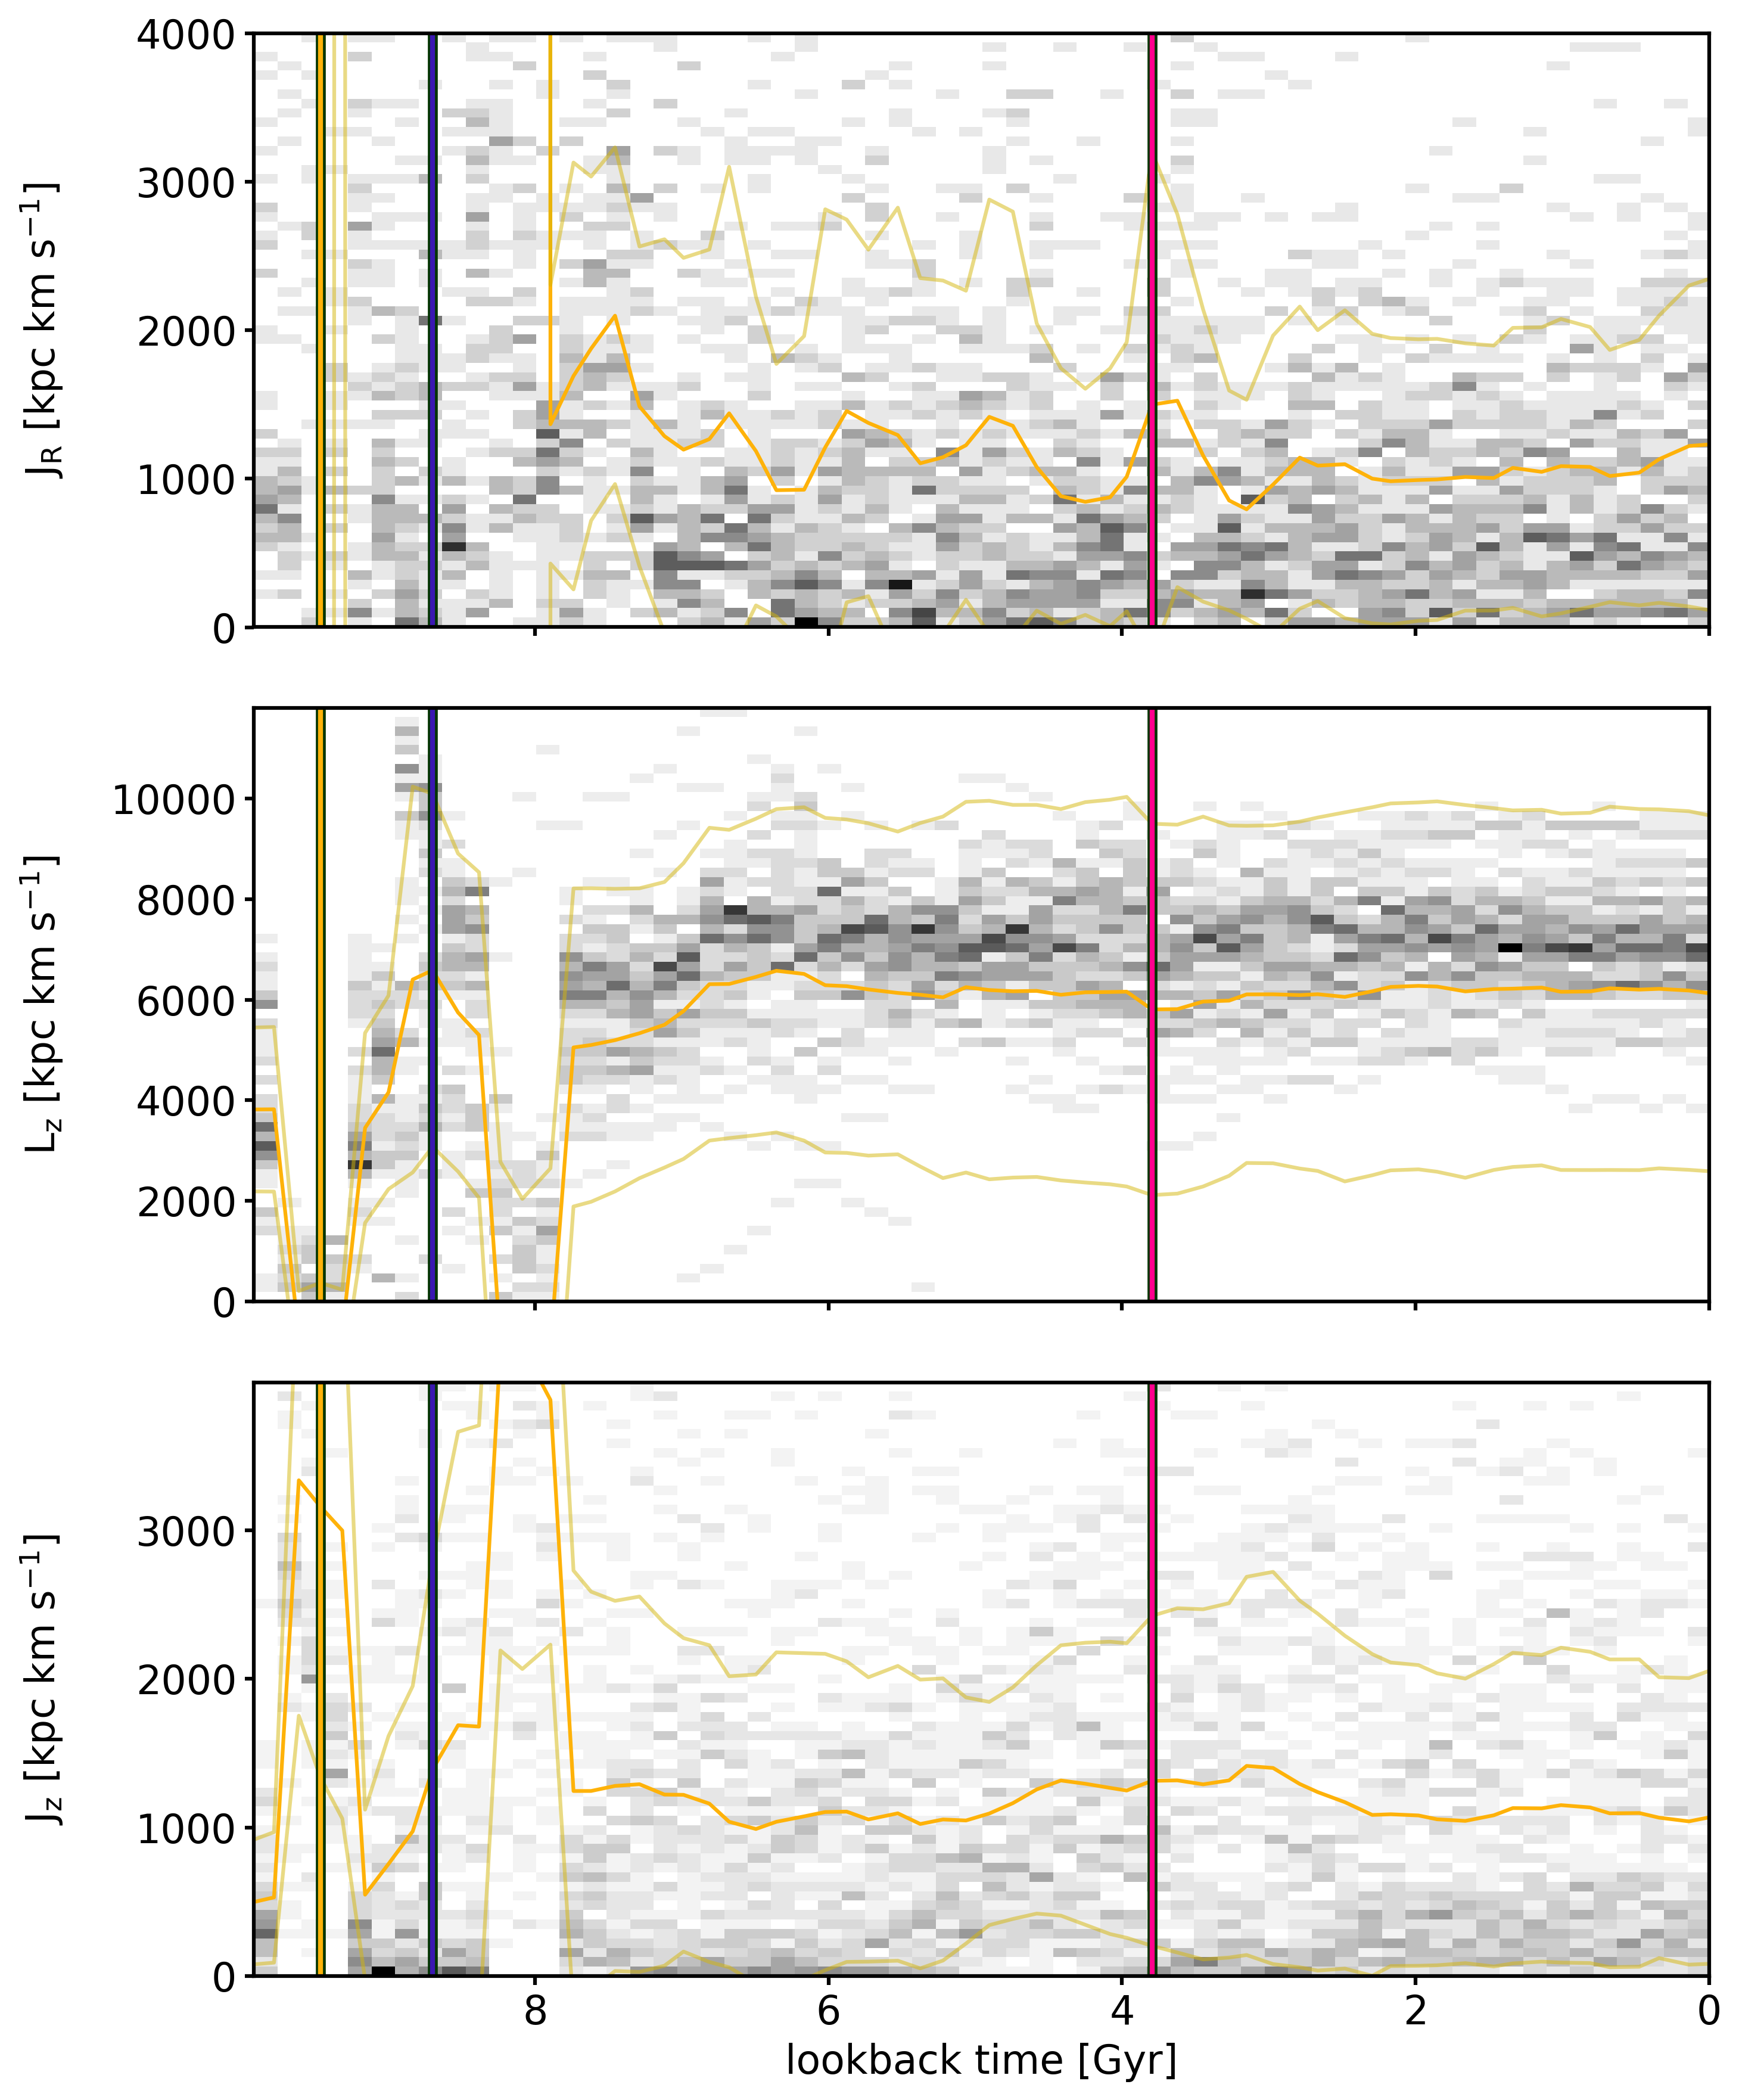
\includegraphics[width=\textwidth]{plots/Dynamics/prog4/action_time_evolution_hist_mean.png}
    \label{fig:time_ev_box_GCs}
    \caption{.}\label{fig:actions_time_evolution}
\end{figure}
